% =====================================================================
%  Rapport de Projet de Fin d'Année (PFA)
%  MCP-Powered BI Ecosystem — Plateforme décisionnelle multi-agents
%  ENSA Oujda — Ingénierie Data Science et Cloud Computing — 2025/2026
%
%  Compatible : pdfLaTeX (Overleaf) ET XeLaTeX / Tectonic.
%  Compilation : `tectonic rapport.tex`  ou  upload sur Overleaf.
% =====================================================================
\documentclass[12pt,a4paper,oneside]{report}

% ---- Moteur : branche pdfTeX vs XeTeX/LuaTeX ------------------------
\usepackage{iftex}
\ifPDFTeX
  \usepackage[utf8]{inputenc}
  \usepackage[T1]{fontenc}
  \usepackage{lmodern}
\else
  \usepackage{fontspec}
\fi

\usepackage[french]{babel}
\frenchsetup{SmallCapsFigTabCaptions=false,AutoSpacePunctuation=true}

% ---- Mise en page ---------------------------------------------------
\usepackage[a4paper,margin=2.5cm,headheight=15pt]{geometry}
\usepackage{setspace}
\onehalfspacing
\usepackage{microtype}

% ---- Couleurs (charte teal/émeraude du projet) ---------------------
\usepackage{xcolor}
\definecolor{accent}{HTML}{0D9488}
\definecolor{accentdark}{HTML}{047857}
\definecolor{accentsoft}{HTML}{D1FAF2}
\definecolor{ink}{HTML}{0F2A30}
\definecolor{muted}{HTML}{5B7178}
\definecolor{codebg}{HTML}{F4F8F7}
\definecolor{codekw}{HTML}{047857}
\definecolor{codestr}{HTML}{B45309}
\definecolor{codecom}{HTML}{8AA0A5}
% Couleurs des accents de la page de garde (marron/terracotta, assorti au logo ENSAO)
\definecolor{coverred}{HTML}{9C5B45}
\definecolor{coverdark}{HTML}{5E3526}
\definecolor{coverpink}{HTML}{E8D2C7}
\definecolor{coverpinklt}{HTML}{F6EAE3}

% ---- Graphiques et schémas -----------------------------------------
\usepackage{graphicx}
\graphicspath{{figures/}{assets/}}
\usepackage{tikz}
\usetikzlibrary{shapes.geometric,arrows.meta,positioning,fit,backgrounds,calc}
\usepackage{caption}
\captionsetup{font=small,labelfont={bf,color=accentdark},margin=10pt}

% ---- Tableaux -------------------------------------------------------
\usepackage{booktabs}
\usepackage{tabularx}
\usepackage{array}
\usepackage{multirow}
\newcolumntype{Y}{>{\raggedright\arraybackslash}X}

% ---- Code source ----------------------------------------------------
\usepackage{listings}
\lstdefinestyle{projet}{
  backgroundcolor=\color{codebg},
  basicstyle=\ttfamily\footnotesize\color{ink},
  keywordstyle=\color{codekw}\bfseries,
  stringstyle=\color{codestr},
  commentstyle=\color{codecom}\itshape,
  numberstyle=\tiny\color{muted},
  numbers=left, numbersep=8pt,
  showstringspaces=false,
  breaklines=true, breakatwhitespace=true,
  frame=single, rulecolor=\color{accentsoft},
  framesep=6pt, xleftmargin=14pt,
  tabsize=2, captionpos=b,
  literate={é}{{\'e}}1 {è}{{\`e}}1 {à}{{\`a}}1 {ê}{{\^e}}1 {ô}{{\^o}}1 {î}{{\^i}}1 {ç}{{\c c}}1 {É}{{\'E}}1 {’}{{'}}1 {→}{{$\rightarrow$}}1 {–}{{-}}1,
}
\lstset{style=projet}
\renewcommand{\lstlistingname}{Extrait de code}

% ---- En-têtes / pieds de page --------------------------------------
\usepackage{fancyhdr}
\pagestyle{fancy}
\fancyhf{}
\fancyhead[L]{\small\nouppercase{\leftmark}}
\fancyhead[R]{\small MCP-Powered BI Ecosystem}
\fancyfoot[C]{\thepage}
\renewcommand{\headrulewidth}{0.4pt}
\renewcommand{\footrulewidth}{0pt}

% Titres de chapitres colorés
\usepackage{titlesec}
\titleformat{\chapter}[display]
  {\normalfont\huge\bfseries\color{accentdark}}
  {\chaptertitlename\ \thechapter}{14pt}{\Huge}
\titlespacing*{\chapter}{0pt}{0pt}{24pt}

% ---- Liens ----------------------------------------------------------
\usepackage[hidelinks]{hyperref}
\hypersetup{
  colorlinks=true, linkcolor=accentdark, urlcolor=accent, citecolor=accent,
  pdftitle={Rapport PFA - MCP-Powered BI Ecosystem},
  pdfauthor={Mohamed Rouane, Zakariae Trachni},
}
\usepackage{enumitem}
\setlist{itemsep=2pt,topsep=3pt}

% ---- Métadonnées du projet (À ADAPTER si besoin) -------------------
\newcommand{\monetablissement}{École Nationale des Sciences Appliquées d'Oujda}
\newcommand{\monuniversite}{Université Mohammed Premier}
\newcommand{\mafiliere}{Ingénierie Data Science et Cloud Computing}
\newcommand{\montitre}{MCP-Powered BI Ecosystem}
\newcommand{\monsoustitre}{Une plateforme décisionnelle généraliste multi-agents orchestrée par le protocole MCP}
\newcommand{\monencadrant}{Pr. Abdelmounaim Kerkri}
\newcommand{\auteurun}{Mohamed Rouane}
\newcommand{\auteurdeux}{Zakariae Trachni}
\newcommand{\monannee}{2025 -- 2026}

% Encadré « callout » réutilisable
\newcommand{\callout}[2]{%
  \begin{center}\begin{minipage}{0.95\linewidth}
  \setlength{\fboxsep}{10pt}%
  \colorbox{accentsoft}{\begin{minipage}{\dimexpr\linewidth-2\fboxsep}
  \textbf{\color{accentdark}#1}\\[2pt]\small #2
  \end{minipage}}
  \end{minipage}\end{center}}

\begin{document}

% ---- Page de garde --------------------------------------------------
% ---- Page de garde (style institutionnel ENSA Oujda) ---------------
\begin{titlepage}
\thispagestyle{empty}
\centering

% --- Fond plein page (vagues rouges) + blocs bas positionnés --------
\begin{tikzpicture}[remember picture,overlay]
  % Image de fond couvrant toute la page
  \node[inner sep=0pt] at (current page.center)
    {
\includegraphics[width=\paperwidth,height=\paperheight]{background.png}};

  % Auteurs (positions fixes, alignés par le haut, au-dessus des vagues)
  \node[anchor=north west,align=left,text=ink,font={\large\linespread{1}\selectfont}]
    at ([xshift=2.4cm,yshift=9.8cm]current page.south west)
    {\textbf{Réalisé par :}\\[4pt]\auteurun\\\auteurdeux};
  \node[anchor=north east,align=right,text=ink,font={\large\linespread{1}\selectfont}]
    at ([xshift=-2.4cm,yshift=9.8cm]current page.south east)
    {\textbf{Encadré par :}\\[4pt]\monencadrant};

  % Membres du jury (centré, sous les auteurs)
  \node[anchor=north,align=center,text=ink,font={\large\linespread{1}\selectfont}] (jurybloc)
    at ([yshift=7.3cm]current page.south)
    {\textbf{Membres du jury :}\\[4pt]Pr. Asmae El Mezouari\\\monencadrant};

  % Année universitaire (écart garanti sous le bloc jury, au-dessus des vagues)
  \node[anchor=north,text=accentdark,font=\large\bfseries,below=0.5cm of jurybloc]
    {Année Universitaire \monannee};
\end{tikzpicture}

\vspace*{0.5cm}

% --- En-tête institutionnel : Français | Logo | Arabe ---------------
\noindent
\begin{minipage}[c]{0.37\textwidth}\centering
  
\includegraphics[height=2.0cm]{entete_fr.png}
\end{minipage}\hfill
\begin{minipage}[c]{0.24\textwidth}\centering
  
\includegraphics[height=2.7cm]{logo_ensa.png}
\end{minipage}\hfill
\begin{minipage}[c]{0.37\textwidth}\centering
  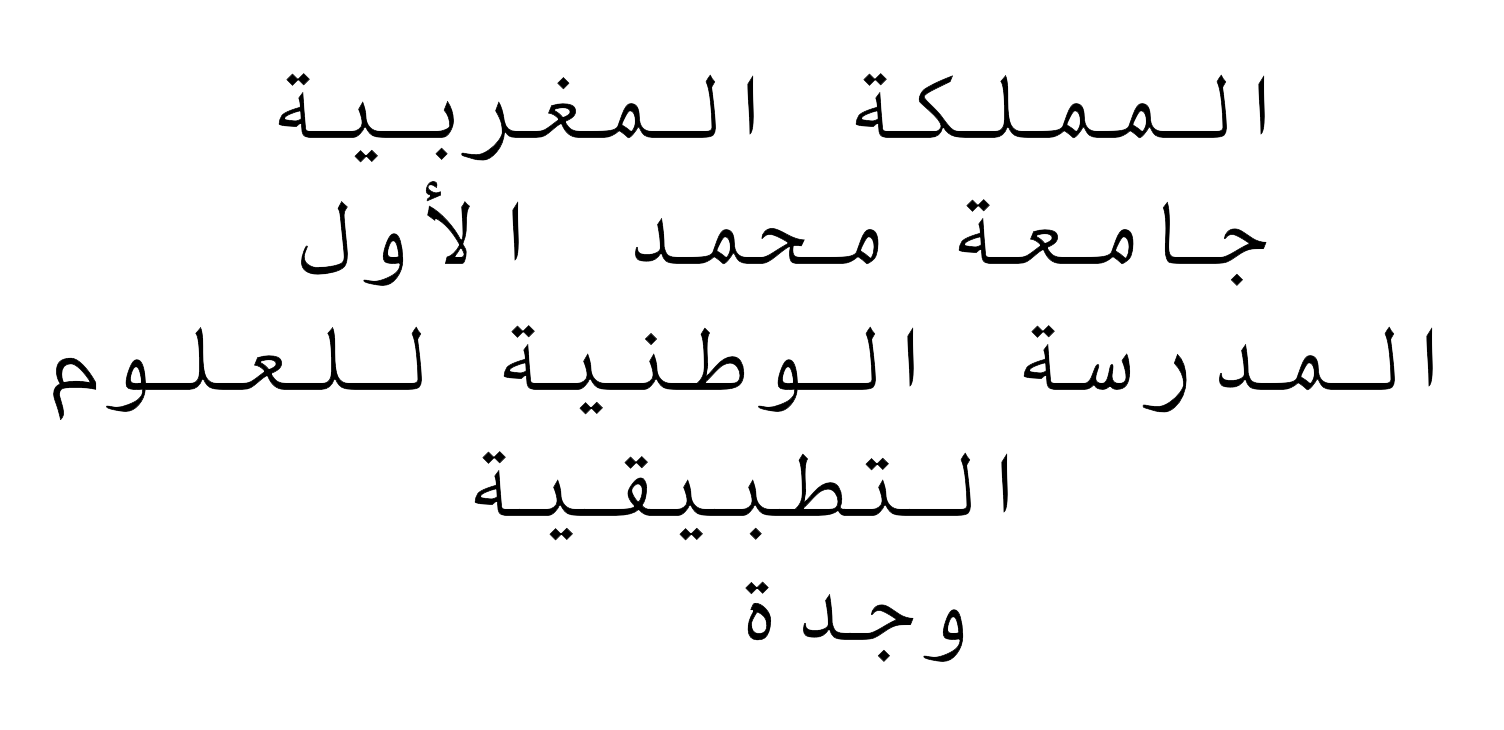
\includegraphics[height=2.0cm]{entete_arabe.png}
\end{minipage}

\vspace{1.1cm}

{\LARGE\scshape École Nationale des Sciences Appliquées\\[2pt] d'Oujda\par}

\vspace{1.3cm}

{\Large\scshape Projet de Fin d'Année (PFA)\par}
\vspace{5pt}
{\large Filière : \mafiliere\par}

\vspace{1.1cm}

% --- Bloc titre encadré de filets rouges ---------------------------
\noindent\textcolor{accentdark}{\rule{\linewidth}{1.4pt}}
\vspace{0.55cm}

{\Huge\bfseries \montitre\par}
\vspace{0.5cm}
{\large\itshape \monsoustitre\par}

\vspace{0.55cm}
\noindent\textcolor{accentdark}{\rule{\linewidth}{1.4pt}}

\vfill
\end{titlepage}


% ---- Pages liminaires (numérotation romaine) -----------------------
\pagenumbering{roman}
% ---- Dédicace -------------------------------------------------------
\chapter*{Dédicace}
\addcontentsline{toc}{chapter}{Dédicace}
\thispagestyle{plain}

\vspace*{1.5cm}
\begin{center}
\textcolor{accent}{\rule{0.32\linewidth}{1.2pt}}\\[1.4cm]
\end{center}

\begin{center}\large\itshape
\setstretch{1.6}
À nos chers \textbf{parents},\\
pour leur amour inconditionnel, leurs sacrifices\\
et leur soutien qui n'a jamais faibli.\\[1.1cm]

À nos \textbf{familles} et à nos \textbf{ami(e)s},\\
pour leurs encouragements constants.\\[1.1cm]

À nos \textbf{enseignants},\\
qui ont éveillé en nous la curiosité\\
et le goût du travail bien fait.\\[1.1cm]

À toutes celles et ceux qui croient\\
qu'une donnée, bien analysée, éclaire la décision.
\end{center}

\vspace{1cm}
\begin{center}
\textcolor{accent}{\rule{0.32\linewidth}{1.2pt}}
\end{center}
\begin{flushright}\itshape
\auteurun\ \& \auteurdeux
\end{flushright}

% ---- Remerciements --------------------------------------------------
\chapter*{Remerciements}
\addcontentsline{toc}{chapter}{Remerciements}

\begin{center}\itshape
« La connaissance s'acquiert par l'expérience, et se transmet par l'exemple. »
\end{center}
\vspace{0.8cm}

Au terme de ce projet de fin d'année, nous tenons à exprimer notre profonde
gratitude à toutes les personnes qui ont rendu ce travail possible.

Nos remerciements les plus sincères s'adressent à notre encadrant,
\textbf{\monencadrant}, qui a su transformer ce projet exigeant en une
expérience formatrice remarquable grâce à :
\begin{itemize}
  \item son \textbf{encadrement rigoureux} et ses orientations éclairées ;
  \item sa \textbf{disponibilité} constante et son écoute attentive ;
  \item ses \textbf{conseils avisés}, déterminants pour nos choix techniques ;
  \item son \textbf{exigence bienveillante}, qui nous a poussés à nous dépasser.
\end{itemize}

Son accompagnement a été déterminant pour :
\begin{itemize}
  \item structurer notre démarche d'ingénierie ;
  \item approfondir notre compréhension des architectures multi-agents ;
  \item mener à bien la réalisation pratique de cette plateforme.
\end{itemize}

Nous adressons également notre reconnaissance :
\begin{itemize}
  \item à l'ensemble du \textbf{corps professoral} de l'\monetablissement,
        pour la qualité de la formation dispensée ;
  \item à nos \textbf{familles}, pour leur soutien indéfectible ;
  \item à nos \textbf{camarades de promotion}, pour leur entraide et leurs
        encouragements.
\end{itemize}

Ce projet a constitué une expérience académique enrichissante, permettant une
application concrète des connaissances théoriques. Nous en garderons non
seulement des compétences techniques solides, mais aussi l'exemple d'un
enseignement de grande qualité.

\vspace{0.8cm}
\begin{flushright}\itshape
Avec toute notre reconnaissance,\\[6pt]
\textbf{\auteurun\ \& \auteurdeux}
\end{flushright}

% ---- Résumé ---------------------------------------------------------
\chapter*{Résumé}
\addcontentsline{toc}{chapter}{Résumé}

Les outils de \textit{Business Intelligence} (BI) traditionnels exigent un
travail manuel important : définition des indicateurs, modélisation des
données, conception des tableaux de bord et rédaction des rapports. Ce
processus est long, coûteux et fortement dépendant d'experts. Ce projet
propose \textbf{\montitre}, une plateforme décisionnelle \emph{généraliste}
et \emph{automatisée} capable d'analyser n'importe quel jeu de données
tabulaire (CSV, Excel, JSON) \emph{sans hypothèse préalable} sur les noms de
colonnes ni sur le domaine métier.

La plateforme repose sur une équipe de \textbf{sept agents d'intelligence
artificielle} spécialisés, orchestrés via le \textbf{protocole MCP} (\textit{Model
Context Protocol}). Un serveur MCP expose, sous forme d'outils contrôlés par
permissions, l'ensemble des capacités du système ; chaque agent (Orchestrateur,
Ingestion, Préparation, KPI, Tableau de bord, Publication, Rédaction) n'a accès
qu'aux outils strictement nécessaires à son rôle. Un \textbf{moteur déterministe
adaptatif} profile automatiquement les données, en déduit des indicateurs et des
visualisations pertinents, tandis que les grands modèles de langage (LLM)
curent, priorisent et rédigent l'analyse. Le système produit, par exécution,
un \textbf{tableau de bord interactif}, un \textbf{rapport décisionnel} (page
web et PDF) et un magasin d'artefacts reproductible.

Des mécanismes de \textbf{fiabilité} ont été conçus : filets de sécurité
déterministes garantissant des livrables complets même en cas de défaillance
d'un agent, vérification automatique des chiffres du rapport face aux
indicateurs calculés, et suivi des coûts (jetons, latence). Une étude de cas
sur un jeu de \textbf{17 769 matchs internationaux de football} valide
l'approche : carte mondiale des buts, détection d'anomalies (dont le match
historique Australie 31--0 Samoa américaines) et mise en évidence de
l'avantage du terrain.

\vspace{6pt}
\noindent\textbf{Mots-clés :} Business Intelligence, agents IA, protocole MCP,
grands modèles de langage, automatisation décisionnelle, visualisation de
données, FastAPI, Plotly.

% ---- Abstract -------------------------------------------------------
\chapter*{Abstract}
\addcontentsline{toc}{chapter}{Abstract}

Traditional Business Intelligence (BI) tools require substantial manual
effort: defining indicators, modelling data, designing dashboards and writing
reports. This process is slow, costly and heavily dependent on experts. This
project introduces \textbf{\montitre}, a \emph{generalist} and \emph{automated}
decision-support platform able to analyse any tabular dataset (CSV, Excel,
JSON) \emph{without prior assumptions} about column names or business domain.

The platform relies on a team of \textbf{seven specialised AI agents}
orchestrated through the \textbf{Model Context Protocol (MCP)}. An MCP server
exposes every capability of the system as permission-controlled tools; each
agent (Orchestrator, Ingestion, Data~Prep, KPI, Dashboard, Publishing,
Reporter) can only access the tools strictly required by its role. A
\textbf{deterministic adaptive engine} automatically profiles the data and
derives relevant indicators and visualisations, while Large Language Models
(LLMs) curate, prioritise and write the analysis. Each run yields an
\textbf{interactive dashboard}, a \textbf{BI report} (web page and PDF) and a
reproducible artifact store.

Reliability mechanisms were designed: deterministic safety nets guaranteeing
complete deliverables even when an agent misbehaves, automatic verification of
the report's figures against the computed indicators, and cost tracking
(tokens, latency). A case study on \textbf{17{,}769 international football
matches} validates the approach: a world map of goals, anomaly detection
(including the historic Australia 31--0 American Samoa match) and the
home-advantage effect.

\vspace{6pt}
\noindent\textbf{Keywords:} Business Intelligence, AI agents, MCP protocol,
Large Language Models, decision automation, data visualisation, FastAPI,
Plotly.

\cleardoublepage


\tableofcontents
\listoffigures
\listoftables
\cleardoublepage

% ---- Corps (numérotation arabe) ------------------------------------
\pagenumbering{arabic}
\setcounter{page}{1}

\chapter*{Introduction générale}
\addcontentsline{toc}{chapter}{Introduction générale}
\markboth{INTRODUCTION GÉNÉRALE}{}

À l'ère du numérique, les organisations produisent et collectent des volumes
de données sans précédent. Transformer ces données brutes en informations
exploitables, puis en décisions éclairées, constitue l'enjeu central de la
\textit{Business Intelligence} (BI). Pourtant, malgré la maturité des outils
du marché (tableurs avancés, plateformes comme Power BI ou Tableau), la
chaîne décisionnelle demeure largement \textbf{manuelle} : un analyste doit
comprendre le schéma des données, choisir les indicateurs clés de performance
(KPI), concevoir des visualisations, puis rédiger un rapport de synthèse.
Chaque nouveau jeu de données relance ce cycle coûteux en temps et en
expertise.

L'émergence des \textbf{grands modèles de langage} (LLM) et des
\textbf{agents d'intelligence artificielle} ouvre la voie à une automatisation
beaucoup plus poussée de cette chaîne. Toutefois, confier l'intégralité de
l'analyse à un modèle de langage se heurte à deux écueils : les modèles
\emph{hallucinent} (ils inventent des chiffres ou des colonnes inexistantes)
et peinent à manipuler de manière fiable des jeux de données volumineux. À
l'inverse, une automatisation purement algorithmique produit des analyses
rigides et dépourvues de discernement métier.

C'est dans cette tension que s'inscrit notre projet de fin d'année. Nous
proposons \textbf{\montitre}, un écosystème décisionnel qui réconcilie ces
deux mondes : un \textbf{moteur déterministe} garantit l'exactitude des
calculs et la robustesse face à n'importe quel schéma de données, tandis
qu'une \textbf{équipe d'agents IA} apporte le jugement, la curation et la
narration. L'ensemble est orchestré par le \textbf{protocole MCP}
(\textit{Model Context Protocol}), un standard récent qui expose les
capacités du système comme un ensemble d'outils contrôlés par permissions et
mobilisables par les agents.

L'originalité de l'approche tient à son caractère \textbf{généraliste} : le
système ne fait \emph{aucune} hypothèse sur le domaine métier. Qu'il s'agisse
de ventes, de logistique, de ressources humaines ou de données sportives, la
plateforme découvre seule la structure des données, en déduit les indicateurs
et visualisations pertinents, puis produit un tableau de bord interactif et un
rapport décisionnel complet.

\section*{Problématique}
Comment concevoir une plateforme de Business Intelligence capable d'analyser
\textbf{automatiquement} et de manière \textbf{fiable} n'importe quel jeu de
données tabulaire, en combinant la rigueur d'un moteur déterministe et le
discernement d'agents fondés sur des modèles de langage, tout en garantissant
la traçabilité, la maîtrise des coûts et la véracité des résultats produits~?

\section*{Objectifs}
Le projet poursuit les objectifs suivants :
\begin{itemize}
  \item concevoir une architecture \textbf{multi-agents} orchestrée par un
        serveur MCP, avec un contrôle d'accès par rôle ;
  \item développer un \textbf{moteur adaptatif} de profilage, de calcul
        d'indicateurs et de génération de visualisations, indépendant du
        domaine métier ;
  \item produire automatiquement un \textbf{tableau de bord interactif} et un
        \textbf{rapport décisionnel} (web et PDF) reproductibles ;
  \item intégrer des mécanismes de \textbf{fiabilité} : filets de sécurité,
        vérification des chiffres, suivi des coûts ;
  \item valider l'approche par une \textbf{étude de cas} réelle.
\end{itemize}

\section*{Organisation du rapport}
Ce rapport s'articule autour de quatre chapitres. Le
\textbf{chapitre~\ref{chap:contexte}} présente le contexte général, la
problématique et l'état de l'art (BI, LLM, agents, protocole MCP). Le
\textbf{chapitre~\ref{chap:conception}} détaille l'analyse des besoins et la
conception de l'architecture. Le \textbf{chapitre~\ref{chap:realisation}}
décrit la réalisation et l'implémentation des différents modules. Enfin, le
\textbf{chapitre~\ref{chap:tests}} expose la stratégie de tests, les
résultats obtenus et une étude de cas approfondie, avant la conclusion et les
perspectives.

\chapter{Contexte général et état de l'art}
\label{chap:contexte}

\callout{En bref}{Ce chapitre situe le projet dans son cadre académique, rappelle
les fondements de la Business Intelligence et de sa chaîne décisionnelle, expose
les limites des outils existants, puis dresse l'état de l'art des briques
technologiques mobilisées : grands modèles de langage, agents d'IA et protocole MCP.}

\section{Cadre du projet}
Ce travail s'inscrit dans le cadre du \textbf{Projet de Fin d'Année (PFA)} de
la filière \textit{\mafiliere} à l'\textbf{\monetablissement}. Le PFA constitue
un jalon pédagogique majeur : il vise à confronter les étudiants à un problème
d'ingingénierie réaliste, à mobiliser de façon intégrée les connaissances
acquises (programmation, science des données, génie logiciel, intelligence
artificielle) et à développer des compétences de conception, de gestion de
projet et de communication scientifique.

Le sujet retenu se situe à l'intersection de trois domaines en pleine
expansion : la \textbf{Business Intelligence}, l'\textbf{ingénierie des données}
et l'\textbf{IA générative}. Il répond à une préoccupation concrète des
organisations : réduire le temps et l'expertise nécessaires pour transformer
des données brutes en connaissances décisionnelles.

\section{La Business Intelligence et la chaîne décisionnelle}

\subsection{Définition et finalité}
La \textbf{Business Intelligence} (informatique décisionnelle) désigne
l'ensemble des méthodes, des processus et des technologies permettant de
collecter, d'organiser, d'analyser et de restituer les données d'une
organisation afin d'éclairer la prise de décision. Son objectif n'est pas la
donnée pour elle-même, mais la \emph{connaissance actionnable} : répondre aux
questions « que s'est-il passé ?\,», « pourquoi ?\,» et « que faire ?\,».

\subsection{La chaîne décisionnelle}
La création de valeur à partir des données suit classiquement une chaîne en
plusieurs maillons, illustrée par la figure~\ref{fig:chaine}.

\begin{figure}[ht]
\centering
\begin{tikzpicture}[
  node distance=4pt and 14pt,
  box/.style={rectangle,rounded corners=4pt,draw=accent,fill=accentsoft,
    text=ink,minimum height=1.3cm,text width=2.4cm,align=center,font=\small\bfseries},
  arr/.style={-{Stealth[length=3mm]},accentdark,thick}]
  \node[box] (a) {Données brutes};
  \node[box,right=of a] (b) {Ingestion \& validation};
  \node[box,right=of b] (c) {Préparation \& nettoyage};
  \node[box,right=of c] (d) {Analyse \& KPIs};
  \node[box,right=of d] (e) {Restitution \& décision};
  \draw[arr] (a)--(b); \draw[arr] (b)--(c); \draw[arr] (c)--(d); \draw[arr] (d)--(e);
\end{tikzpicture}
\caption{La chaîne décisionnelle classique de la Business Intelligence.}
\label{fig:chaine}
\end{figure}

Chaque maillon mobilise des savoir-faire distincts :
\begin{itemize}
  \item \textbf{Ingestion} : récupération des données depuis des sources
        hétérogènes (fichiers, bases de données, API) et contrôle de leur
        intégrité ;
  \item \textbf{Préparation} : nettoyage, traitement des valeurs manquantes,
        typage, normalisation ;
  \item \textbf{Analyse} : définition et calcul des indicateurs clés de
        performance (KPI), exploration statistique ;
  \item \textbf{Restitution} : conception de tableaux de bord et de rapports
        destinés aux décideurs.
\end{itemize}

\subsection{Notions d'indicateurs, dimensions et mesures}
La modélisation décisionnelle distingue traditionnellement les
\textbf{mesures} (grandeurs numériques agrégeables : chiffre d'affaires,
quantités, buts marqués) des \textbf{dimensions} (axes d'analyse catégoriels
ou temporels : région, produit, date) selon lesquels les mesures sont
ventilées. Un \textbf{KPI} (\textit{Key Performance Indicator}) est une
mesure synthétique, souvent agrégée selon une ou plusieurs dimensions,
choisie pour sa pertinence métier. Cette distinction, fondamentale, est au
cœur de l'approche adaptative développée dans ce projet
(chapitre~\ref{chap:realisation}).

\section{Problématique : les limites des outils BI classiques}
Malgré leur richesse fonctionnelle, les solutions de BI du marché présentent
plusieurs limites structurantes :

\begin{description}
  \item[Forte dépendance à l'expertise.] La conception d'un tableau de bord
    pertinent suppose une bonne compréhension métier \emph{et} technique.
    L'analyste reste un goulot d'étranglement.
  \item[Travail répétitif et chronophage.] Chaque nouveau jeu de données
    impose de reparcourir la chaîne décisionnelle : exploration, choix des
    indicateurs, construction des graphiques, rédaction.
  \item[Spécialisation par cas d'usage.] Les solutions sont souvent
    paramétrées pour un domaine précis (BI commerciale, BI RH), avec des
    hypothèses figées sur la nature des colonnes.
  \item[Restitution manuelle.] La rédaction du rapport narratif — pourtant
    essentielle à la décision — demeure entièrement humaine.
\end{description}

Ces limites motivent la recherche d'une plateforme \textbf{généraliste} et
\textbf{automatisée}, capable de s'adapter à n'importe quel schéma de données
et de produire, sans intervention humaine, l'ensemble des livrables
décisionnels. Le tableau~\ref{tab:comparaison} synthétise l'écart entre
l'approche traditionnelle et celle que nous proposons.

\begin{table}[ht]
\centering\small
\caption{Comparaison entre la BI traditionnelle et l'approche proposée.}
\label{tab:comparaison}
\begin{tabularx}{\linewidth}{@{}lYY@{}}
\toprule
\textbf{Critère} & \textbf{BI traditionnelle} & \textbf{Approche proposée} \\
\midrule
Choix des KPIs & Manuel, par un expert & Automatique et adaptatif \\
Conception des graphiques & Manuelle & Automatique selon les rôles \\
Rédaction du rapport & Humaine & Générée par agents IA \\
Adaptation au domaine & Paramétrage spécifique & Aucune hypothèse métier \\
Délai d'obtention & Heures à jours & Quelques secondes \\
Véracité des chiffres & Confiance humaine & Vérification automatique \\
\bottomrule
\end{tabularx}
\end{table}

\section{Objectifs et périmètre}
Le périmètre du projet couvre l'intégralité de la chaîne décisionnelle, de
l'ingestion d'un fichier tabulaire jusqu'à la production d'un rapport
décisionnel. Les choix structurants sont les suivants :
\begin{itemize}
  \item support des formats \texttt{CSV}, \texttt{Excel} et \texttt{JSON} ;
  \item \textbf{aucune} configuration spécifique au domaine métier ;
  \item génération automatique d'un tableau de bord interactif et d'un
        rapport (web + PDF) ;
  \item exécution locale, reproductible, avec un magasin d'artefacts par
        exécution.
\end{itemize}
Sont hors périmètre : la connexion temps réel à des bases de données de
production, la gestion multi-utilisateurs et le déploiement à l'échelle, qui
constituent des perspectives (voir la conclusion générale).

\section{État de l'art}

\subsection{Les grands modèles de langage (LLM)}
Un \textbf{grand modèle de langage} est un réseau de neurones, fondé sur
l'architecture \textit{Transformer}~\cite{vaswani2017attention}, entraîné sur
d'immenses corpus textuels pour prédire le mot suivant. Au-delà de la
génération de texte, ces modèles manifestent des capacités de raisonnement, de
synthèse et de \emph{suivi d'instructions}. Une avancée déterminante pour notre
projet est l'\textbf{appel d'outils} (\textit{tool use} / \textit{function
calling})~: le modèle peut décider d'invoquer une fonction externe avec des
arguments structurés, puis exploiter le résultat. C'est précisément ce
mécanisme qui permet à un LLM de piloter un système logiciel plutôt que de se
contenter de produire du texte.

Nous mobilisons des modèles performants tels que \textbf{Llama~3.3}~\cite{llama3}
servis par l'infrastructure \textbf{Groq} (inférence à très faible latence), ou
des modèles exécutés localement via \textbf{Ollama}. Les LLM présentent
néanmoins deux faiblesses notoires : la tendance à l'\textbf{hallucination}
(production d'informations erronées mais plausibles) et la difficulté à
manipuler fidèlement de grandes tables. Ces limites guident notre choix
architectural : confier les calculs à un moteur déterministe et réserver aux
LLM la curation et la rédaction.

\subsection{Les agents d'intelligence artificielle}
Un \textbf{agent} est un système qui perçoit un environnement, raisonne et
agit pour atteindre un objectif. Appliqué aux LLM, le paradigme agentique
consiste à doter un modèle d'une \textbf{boucle} : observer l'état, décider
d'une action (souvent un appel d'outil), exécuter, observer le résultat, et
recommencer jusqu'à l'accomplissement de la tâche. Les approches multi-agents
décomposent un problème complexe en \textbf{rôles spécialisés} qui coopèrent,
à l'image d'une équipe humaine. Cette spécialisation améliore la fiabilité,
la lisibilité et la maintenabilité, chaque agent disposant d'un contexte et
de permissions restreints à sa mission.

\subsection{Le protocole MCP (Model Context Protocol)}
Le \textbf{Model Context Protocol}~\cite{mcp} est un standard ouvert,
introduit par Anthropic, qui normalise la manière dont une application expose
ses \textbf{outils}, ses \textbf{ressources} et ses \textbf{données} à des
modèles de langage. À la manière d'un « port universel » entre les LLM et le
monde logiciel, MCP définit un format commun pour décrire un outil (nom,
description, schéma JSON des arguments) et pour l'invoquer.

Dans notre projet, MCP joue un double rôle structurant : il sert de
\textbf{registre central des capacités} du système (chargement de données,
profilage, calcul d'indicateurs, génération de graphiques, etc.) et de
\textbf{mécanisme de contrôle d'accès}. Chaque agent se voit attribuer un
sous-ensemble d'outils autorisés ; toute tentative d'appel hors de ce
périmètre est refusée par le serveur. Ce principe de \emph{moindre privilège}
renforce la sûreté et clarifie les responsabilités.

\subsection{Modélisation dimensionnelle et entrepôts de données}
La théorie de la \textbf{modélisation dimensionnelle}, formalisée notamment par
Kimball~\cite{kimball2013}, structure les données décisionnelles autour de
\emph{tables de faits} (contenant les mesures) et de \emph{tables de dimensions}
(contenant les axes d'analyse). Cette séparation conceptuelle entre
\textbf{faits/mesures} et \textbf{dimensions} irrigue directement notre moteur de
profilage : plutôt que d'imposer un schéma en étoile prédéfini, le système
\emph{infère} dynamiquement le rôle de chaque colonne. Cette inférence
automatique des rôles constitue la transposition « sans configuration » des
principes de la modélisation dimensionnelle à un contexte généraliste.

\subsection{Outils de visualisation et frameworks web}
La restitution s'appuie sur \textbf{Plotly}~\cite{plotly}, une bibliothèque de
visualisation interactive produisant des graphiques en HTML/JavaScript
autonomes, et sur \textbf{FastAPI}~\cite{fastapi}, un framework web Python
moderne et performant pour l'interface utilisateur. La manipulation des
données repose sur \textbf{pandas}~\cite{pandas}, référence de l'analyse de
données tabulaires en Python.

\section{Méthodologie de travail}
Le projet a été conduit selon une démarche \textbf{itérative et incrémentale}.
Une première itération a établi le socle (moteur déterministe, serveur MCP,
sept agents, interface) ; les itérations suivantes ont enrichi le système
(robustesse, vérification des chiffres, suivi des coûts, cartes
géographiques, détection d'anomalies, comparaison de segments) et amélioré
l'interface. Chaque incrément a été \textbf{validé par des tests}
automatisés et par des exécutions de bout en bout sur des jeux de données
réels, garantissant la non-régression. Cette approche a permis de livrer en
permanence un système fonctionnel et de prioriser les fonctionnalités à plus
forte valeur.

\section{Gestion et planification du projet}
Le projet a été planifié en \textbf{cinq phases} successives mais partiellement
recouvrantes, conformément à la démarche itérative. La
figure~\ref{fig:gantt} en présente le diagramme de Gantt simplifié.

\begin{figure}[ht]
\centering
\begin{tikzpicture}[x=0.95cm,y=0.62cm,font=\footnotesize]
  % axe temps (semaines)
  \foreach \x in {0,...,12} \draw[muted!40] (\x,0.4) -- (\x,-5.2);
  \foreach \x/\lab in {0/S1,2/S3,4/S5,6/S7,8/S9,10/S11,12/S13}
     \node[muted,font=\scriptsize] at (\x,0.8) {\lab};
  % barres : nom, debut, duree, ligne
  \def\bar#1#2#3#4{\fill[accent,rounded corners=2pt] (#2,-#4+0.2) rectangle (#2+#3,-#4-0.2);
     \node[anchor=east,text=ink] at (-0.2,-#4) {#1};}
  \bar{Étude \& état de l'art}{0}{2.5}{1}
  \bar{Conception}{2}{2.5}{2}
  \bar{Développement du socle}{3.5}{4}{3}
  \bar{Enrichissement \& fiabilité}{7}{4}{4}
  \bar{Tests \& rédaction}{9.5}{3}{5}
\end{tikzpicture}
\caption{Diagramme de Gantt simplifié du déroulement du projet.}
\label{fig:gantt}
\end{figure}

\begin{description}
  \item[Étude \& état de l'art.] Cadrage du sujet, revue des concepts (BI, LLM,
    agents, MCP) et choix technologiques.
  \item[Conception.] Définition des besoins, de l'architecture en couches et
    de la répartition des rôles entre agents.
  \item[Développement du socle.] Moteur déterministe, serveur MCP, sept agents,
    interface web et premier pipeline de bout en bout.
  \item[Enrichissement \& fiabilité.] Filets de sécurité, vérification des
    chiffres, suivi des coûts, cartes géographiques et analyses avancées.
  \item[Tests \& rédaction.] Consolidation des tests, étude de cas et rédaction
    du présent rapport.
\end{description}

\callout{Synthèse du chapitre}{La BI traditionnelle reste manuelle, coûteuse et
spécialisée. Les LLM et les agents, couplés au protocole MCP, offrent les briques
d'une automatisation généralisée — à condition d'en maîtriser les faiblesses
(hallucinations, fiabilité). Le chapitre suivant traduit ce constat en une
architecture concrète.}

\chapter{Analyse et conception}
\label{chap:conception}

\callout{En bref}{Ce chapitre formalise les besoins, présente l'architecture
en couches du système, détaille le serveur MCP et son registre d'outils
permissionné, décrit les sept agents et leur matrice de permissions, expose le
moteur déterministe adaptatif, et illustre la conception par des diagrammes UML.}

\section{Spécification des besoins}

\subsection{Besoins fonctionnels}
Le système doit permettre à un utilisateur de :
\begin{enumerate}
  \item \textbf{téléverser} un jeu de données tabulaire (CSV, Excel, JSON) ;
  \item déclencher une \textbf{analyse automatique} de bout en bout ;
  \item suivre en \textbf{temps réel} l'avancement du traitement par étape ;
  \item consulter un \textbf{tableau de bord interactif} (indicateurs et
        graphiques) ;
  \item consulter et \textbf{exporter} un \textbf{rapport décisionnel}
        (page web, PDF, HTML) ;
  \item retrouver et rouvrir les \textbf{exécutions passées} et leurs
        artefacts.
\end{enumerate}

\subsection{Besoins non fonctionnels}
\begin{description}
  \item[Généralité.] Le système ne doit faire aucune hypothèse sur le domaine
    métier ni sur les noms de colonnes.
  \item[Fiabilité.] Une exécution doit toujours produire des livrables
    complets, même en cas de défaillance d'un agent.
  \item[Véracité.] Les chiffres du rapport doivent être vérifiables face aux
    indicateurs effectivement calculés.
  \item[Sûreté.] Chaque agent ne doit accéder qu'aux outils nécessaires à son
    rôle (moindre privilège).
  \item[Reproductibilité.] Chaque exécution doit être tracée dans un magasin
    d'artefacts autonome.
  \item[Observabilité.] La consommation (jetons, latence, coût estimé) doit
    être mesurée et restituée.
  \item[Portabilité.] Le système doit fonctionner avec un fournisseur de LLM
    hébergé (Groq) ou local (Ollama).
\end{description}

\subsection{Acteurs et cas d'usage}
L'acteur principal est l'\textbf{Analyste / Décideur}, qui interagit avec la
plateforme via une interface web. La figure~\ref{fig:usecase} présente le
diagramme de cas d'usage.

\begin{figure}[ht]
\centering
\begin{tikzpicture}[
  uc/.style={ellipse,draw=accent,fill=accentsoft,text=ink,minimum width=4.3cm,
    minimum height=1.05cm,align=center,font=\small,inner sep=1pt},
  line/.style={accentdark,thick}]
  % --- Acteur (stick figure soigné) ---
  \begin{scope}[shift={(-4.4,-3.0)},accentdark,line width=1.2pt]
    \draw[fill=accentsoft] (0,1) circle (0.34);        % tête
    \draw (0,0.66) -- (0,-0.55);                        % tronc
    \draw (-0.55,0.28) -- (0.55,0.28);                  % bras
    \draw (0,-0.55) -- (-0.45,-1.3);                    % jambe gauche
    \draw (0,-0.55) -- (0.45,-1.3);                     % jambe droite
  \end{scope}
  \node[font=\small\bfseries,text=ink] at (-4.4,-4.55) {Analyste};
  \node[font=\scriptsize,text=muted] at (-4.4,-4.95) {/ Décideur};

  % --- Frontière du système ---
  \node[draw=accent,line width=1pt,rounded corners=8pt,fill=accent!3,
        minimum width=7.8cm,minimum height=8.4cm,
        label={[font=\small\bfseries,text=accentdark,yshift=-2pt]north:Plateforme BI multi-agents}]
        (sys) at (2.2,-3.0) {};

  % --- Cas d'usage (répartis verticalement) ---
  \node[uc] (u1) at (2.2,-0.5) {Téléverser un jeu de données};
  \node[uc] (u2) at (2.2,-1.75) {Lancer une analyse automatique};
  \node[uc] (u3) at (2.2,-3.0) {Suivre la progression};
  \node[uc] (u4) at (2.2,-4.25) {Consulter le tableau de bord};
  \node[uc] (u5) at (2.2,-5.5) {Consulter / exporter le rapport};

  % --- Liens acteur -> cas d'usage ---
  \foreach \u in {u1,u2,u3,u4,u5} \draw[line] (-3.7,-3.0) -- (\u.west);
\end{tikzpicture}
\caption{Diagramme de cas d'usage de la plateforme.}
\label{fig:usecase}
\end{figure}

\section{Architecture globale}
L'architecture adopte une organisation \textbf{en couches} (figure~\ref{fig:archi}),
qui sépare nettement les responsabilités et permet une évolution
indépendante de chaque niveau.

\begin{figure}[ht]
\centering
\begin{tikzpicture}[
  L/.style={rounded corners=5pt, draw=accent, line width=0.8pt,
    minimum width=10.2cm, minimum height=1.05cm, text width=9.3cm,
    align=left, font=\small, inner xsep=11pt, inner ysep=6pt},
  down/.style={-{Stealth[length=3mm]}, accentdark, line width=1.4pt},
  back/.style={-{Stealth[length=3mm]}, accent, line width=1pt, dashed}]

  \node[L, fill=accent, text=white] (ui)
    {\textbf{Couche présentation}\\[1pt]{\scriptsize Interface web FastAPI — téléversement, suivi, tableau de bord, rapport}};
  \node[L, fill=accentsoft, below=7mm of ui] (orch)
    {\textbf{Couche orchestration}\\[1pt]{\scriptsize Pipeline + filets de sécurité déterministes}};
  \node[L, fill=accentsoft, below=7mm of orch] (ag)
    {\textbf{Couche agents}\\[1pt]{\scriptsize Orchestrateur · Ingestion · Data Prep · KPI · Dashboard · Publication · Reporter}};
  \node[L, fill=accentdark, text=white, below=7mm of ag] (mcp)
    {\textbf{Serveur MCP}\\[1pt]{\scriptsize Registre de 14 outils + contrôle d'accès par rôle (refus par défaut)}};
  \node[L, fill=accentsoft, below=7mm of mcp] (core)
    {\textbf{Moteur déterministe}\\[1pt]{\scriptsize Profilage · KPIs · Graphiques · Insights · Validation}};
  \node[L, fill=white, below=7mm of core] (store)
    {\textbf{Magasin d'artefacts}\\[1pt]{\scriptsize \texttt{dashboard.html} · \texttt{report.html} · \texttt{state.json}}};

  % Flux descendant : la requête traverse les couches
  \foreach \a/\b in {ui/orch, orch/ag, ag/mcp, mcp/core, core/store}
    \draw[down] (\a) -- (\b);

  % Flux remontant : les résultats reviennent vers l'interface
  \draw[back] (store.east) .. controls +(2.2,0) and +(2.2,0) .. (ui.east)
    node[pos=0.5, fill=white, inner sep=1.5pt, text=muted, font=\scriptsize] {résultats};
\end{tikzpicture}
\caption{Architecture en couches du système.}
\label{fig:archi}
\end{figure}

Le principe directeur est une \textbf{séparation des préoccupations} :
\begin{itemize}
  \item la \textbf{présentation} (interface web) ne contient aucune logique
        d'analyse ;
  \item l'\textbf{orchestration} séquence les agents et garantit la complétude
        des résultats ;
  \item les \textbf{agents} portent le jugement métier (curation, narration) ;
  \item le \textbf{serveur MCP} médie tous les accès aux capacités et applique
        les permissions ;
  \item le \textbf{moteur déterministe} effectue tous les calculs ;
  \item le \textbf{magasin d'artefacts} assure la traçabilité.
\end{itemize}

\section{Le serveur MCP et le registre d'outils}
Le serveur MCP est le \textbf{point de passage obligé} entre les agents et les
capacités du système. Il expose 14 \textbf{outils}, chacun décrit par un nom,
une description en langage naturel et un \textbf{schéma JSON} de ses arguments
— description directement exploitable par les LLM pour décider de leurs appels.
Le tableau~\ref{tab:outils} récapitule ces outils.

\begin{table}[ht]
\centering\small
\caption{Les outils exposés par le serveur MCP.}
\label{tab:outils}
\begin{tabularx}{\linewidth}{@{}lY@{}}
\toprule
\textbf{Outil} & \textbf{Rôle} \\
\midrule
\texttt{load\_dataset} & Charge un fichier (CSV/Excel/JSON) et l'enregistre. \\
\texttt{validate\_dataset} & Contrôle structurel (doublons, colonnes vides…). \\
\texttt{profile\_dataset} & Profile les colonnes (rôles, cardinalité, statistiques). \\
\texttt{clean\_dataset} & Applique des opérations de nettoyage. \\
\texttt{suggest\_kpis} / \texttt{compute\_kpis} & Propose puis calcule les indicateurs. \\
\texttt{detect\_anomalies} & Détecte les valeurs aberrantes et pics temporels. \\
\texttt{compare\_segments} & Compare une mesure entre groupes. \\
\texttt{suggest\_charts} / \texttt{build\_chart} & Propose puis construit les graphiques. \\
\texttt{build\_dashboard} & Assemble le tableau de bord interactif. \\
\texttt{publish\_artifacts} & Fige l'état de l'exécution sur disque. \\
\texttt{generate\_report} & Produit le rapport décisionnel (HTML). \\
\texttt{get\_run\_state} / \texttt{set\_run\_state} & Lit / écrit l'état partagé de l'exécution. \\
\bottomrule
\end{tabularx}
\end{table}

\section{Les sept agents et la matrice de permissions}
Le système répartit le travail entre \textbf{sept agents spécialisés}. Chaque
agent possède un \textbf{rôle}, une \textbf{invite système} (\textit{prompt})
qui le cadre, et un \textbf{ensemble d'outils autorisés} défini dans le
fichier de configuration \texttt{config.yaml}. Le serveur MCP applique ces
permissions à chaque appel, selon un principe de \textbf{refus par défaut}.
Le tableau~\ref{tab:permissions} présente cette matrice.

\begin{table}[ht]
\centering\small
\caption{Matrice rôles / permissions (extraite de \texttt{config.yaml}).}
\label{tab:permissions}
\begin{tabularx}{\linewidth}{@{}lY@{}}
\toprule
\textbf{Agent} & \textbf{Outils autorisés} \\
\midrule
\textbf{Orchestrateur} & \texttt{list\_agents}, \texttt{get\_run\_state}, \texttt{set\_run\_state} \\
\textbf{Ingestion} & \texttt{load\_dataset}, \texttt{validate\_dataset} \\
\textbf{Data Prep} & \texttt{profile\_dataset}, \texttt{clean\_dataset} \\
\textbf{KPI} & \texttt{profile\_dataset}, \texttt{suggest\_kpis}, \texttt{compute\_kpis}, \texttt{detect\_anomalies}, \texttt{compare\_segments} \\
\textbf{Dashboard} & \texttt{profile\_dataset}, \texttt{suggest\_charts}, \texttt{build\_chart} \\
\textbf{Publication} & \texttt{build\_dashboard}, \texttt{publish\_artifacts} \\
\textbf{Reporter} & \texttt{get\_run\_state}, \texttt{generate\_report} \\
\bottomrule
\end{tabularx}
\end{table}

\subsection{Rôles des agents}
\begin{description}
  \item[Orchestrateur.] Planifie l'exécution, observe la forme des données et
    signale les risques. Il ne manipule pas directement les données.
  \item[Ingestion.] Charge le fichier brut et valide sa structure.
  \item[Data Prep.] Profile les colonnes et applique un nettoyage minimal et
    sûr.
  \item[KPI.] Sélectionne, parmi des candidats adaptatifs, les indicateurs les
    plus pertinents, les calcule, puis détecte anomalies et écarts de segments.
  \item[Dashboard.] Choisit un ensemble équilibré de graphiques et les
    construit.
  \item[Publication.] Assemble le tableau de bord HTML et fige les artefacts.
  \item[Reporter.] Rédige le rapport décisionnel en s'appuyant exclusivement
    sur l'état réel de l'exécution.
\end{description}

\subsection{Boucle d'exécution d'un agent}
Chaque agent fonctionne selon une \textbf{boucle d'appel d'outils} bornée :
le LLM reçoit l'invite et la liste de ses outils autorisés, décide d'un ou
plusieurs appels, le serveur MCP exécute et renvoie les résultats, puis le
modèle poursuit jusqu'à produire une réponse finale. Un mécanisme de
\textbf{relance avec incitation} (\textit{retry-with-nudge}) corrige le cas
fréquent où le modèle répond par du texte sans appeler ses outils.

\section{Le moteur déterministe adaptatif}
Le cœur « intelligent » généraliste ne peut reposer entièrement sur le LLM :
face à des dizaines de colonnes, le modèle hallucinerait des noms et
manquerait des agrégations évidentes. Le \textbf{moteur déterministe} produit
donc une base adaptative riche, que les agents \emph{curent} et \emph{narrent}.

\subsection{Profilage par rôles}
Le profileur classe chaque colonne dans un \textbf{rôle sémantique} :
\textbf{mesure} (numérique agrégeable), \textbf{dimension} (catégorielle de
faible cardinalité), \textbf{date}, \textbf{identifiant}, \textbf{texte},
\textbf{booléen}, ou \textbf{géographie} (valeurs reconnues comme des pays).
Ces rôles, déduits par des heuristiques paramétrables, permettent à tout le
reste du système d'agir de manière générique.

\subsection{Génération adaptative}
À partir des seuls rôles, le moteur dérive :
\begin{itemize}
  \item des \textbf{KPIs} candidats (totaux, moyennes, comptages distincts,
        variation période sur période, part du segment dominant) ;
  \item des \textbf{graphiques} candidats (séries temporelles, barres top-N,
        distributions, nuages de points, parts, carte choroplèthe, heatmap de
        corrélations) ;
  \item des \textbf{insights} (anomalies, comparaisons de segments,
        corrélations).
\end{itemize}

\section{Diagrammes de conception}
La figure~\ref{fig:sequence} présente le diagramme de séquence simplifié d'une
exécution, mettant en évidence l'orchestration des sept agents via le serveur
MCP.

\begin{figure}[ht]
\centering
\begin{tikzpicture}[font=\scriptsize,
  life/.style={thick,muted,dashed},
  msg/.style={-{Stealth[length=2mm]},accentdark},
  head/.style={rectangle,rounded corners=3pt,draw=accent,fill=accentsoft,
    text=ink,minimum width=1.7cm,minimum height=0.7cm,align=center,font=\scriptsize\bfseries}]
  % lifelines
  \node[head] (U) at (0,0) {Utilisateur};
  \node[head] (P) at (2.6,0) {Pipeline};
  \node[head] (A) at (5.2,0) {Agents};
  \node[head] (M) at (7.8,0) {Serveur MCP};
  \node[head] (C) at (10.4,0) {Moteur};
  \foreach \n in {U,P,A,M,C} \draw[life] (\n.south) -- ++(0,-7.4);
  % messages
  \def\y{-0.7}
  \draw[msg] (U.south|-0,\y) -- node[above]{téléverse} (P.south|-0,\y);
  \def\y{-1.5}\draw[msg] (P.south|-0,\y) -- node[above]{lance étape} (A.south|-0,\y);
  \def\y{-2.3}\draw[msg] (A.south|-0,\y) -- node[above]{appelle outil} (M.south|-0,\y);
  \def\y{-3.1}\draw[msg] (M.south|-0,\y) -- node[above]{exécute} (C.south|-0,\y);
  \def\y{-3.9}\draw[msg] (C.south|-0,\y) -- node[above]{résultat} (M.south|-0,\y);
  \def\y{-4.7}\draw[msg] (M.south|-0,\y) -- node[above]{renvoie} (A.south|-0,\y);
  \def\y{-5.5}\draw[msg] (A.south|-0,\y) -- node[above]{état mis à jour} (P.south|-0,\y);
  \def\y{-6.6}\draw[msg] (P.south|-0,\y) -- node[above]{artefacts (dashboard, rapport)} (U.south|-0,\y);
  \node[text=muted] at (5.2,-7.0) {\footnotesize\itshape Répété pour les 7 agents : Ingestion → Orchestrateur → Data Prep → KPI → Dashboard → Publication → Reporter};
\end{tikzpicture}
\caption{Diagramme de séquence simplifié d'une exécution du pipeline.}
\label{fig:sequence}
\end{figure}

\subsection{Vue en composants}
La figure~\ref{fig:composants} présente l'organisation en composants
logiciels et leurs dépendances. Le pipeline dépend des agents, qui dépendent
tous du serveur MCP ; celui-ci est le seul à dépendre du moteur déterministe
et du client LLM. Cette dépendance \emph{en entonnoir} matérialise le rôle de
médiateur unique du serveur MCP.

\begin{figure}[ht]
\centering
\begin{tikzpicture}[
  comp/.style={rectangle,draw=accent,fill=white,text=ink,rounded corners=3pt,
    minimum height=0.95cm,minimum width=2.7cm,align=center,font=\scriptsize\bfseries},
  pkg/.style={rectangle,draw=accentdark,fill=accentsoft,text=ink,rounded corners=3pt,
    minimum height=0.95cm,minimum width=2.7cm,align=center,font=\scriptsize\bfseries},
  dep/.style={-{Stealth[length=2.2mm]},muted,thick}]
  \node[comp] (ui) at (0,4) {ui\\(FastAPI)};
  \node[comp] (pipe) at (0,2.6) {pipeline.py};
  \node[comp] (agents) at (0,1.2) {agents\\(7 agents)};
  \node[pkg] (mcp) at (0,-0.3) {mcp\_server\\(outils + perms)};
  \node[pkg] (core) at (-2.9,-2.0) {core\\(moteur)};
  \node[pkg] (llm) at (2.9,-2.0) {llm\\(Groq/Ollama)};
  \node[comp] (store) at (0,-3.6) {Magasin\\d'artefacts};
  \draw[dep] (ui)--(pipe); \draw[dep] (pipe)--(agents); \draw[dep] (agents)--(mcp);
  \draw[dep] (mcp)--(core); \draw[dep] (mcp)--(llm);
  \draw[dep] (agents.east) to[bend left=30] (llm.north);
  \draw[dep] (core)--(store); \draw[dep] (mcp)--(store);
\end{tikzpicture}
\caption{Diagramme de composants et dépendances.}
\label{fig:composants}
\end{figure}

\callout{Synthèse du chapitre}{L'architecture en couches isole présentation,
orchestration, agents, serveur MCP, moteur et artefacts. Le serveur MCP
centralise 14 outils et applique une matrice de permissions stricte aux sept
agents. Le moteur déterministe garantit la généralité ; les agents apportent le
jugement. Le chapitre suivant détaille la réalisation.}

\chapter{Réalisation et implémentation}
\label{chap:realisation}

\callout{En bref}{Ce chapitre décrit la mise en œuvre concrète du système :
l'environnement technique, le profilage adaptatif, le calcul des indicateurs,
les visualisations (dont la carte géographique), les analyses avancées
(anomalies, segments), l'orchestration avec ses filets de sécurité, la
publication des livrables et les mécanismes de fiabilité.}

\section{Environnement et technologies}
Le système est développé en \textbf{Python~3}. Le tableau~\ref{tab:tech}
récapitule les principales technologies et leur rôle.

\begin{table}[ht]
\centering\small
\caption{Technologies utilisées.}
\label{tab:tech}
\begin{tabularx}{\linewidth}{@{}lY@{}}
\toprule
\textbf{Technologie} & \textbf{Rôle dans le projet} \\
\midrule
\textbf{pandas / NumPy} & Manipulation et analyse des données tabulaires. \\
\textbf{Plotly} & Génération des graphiques interactifs (HTML autonome). \\
\textbf{FastAPI / Uvicorn} & Interface web (téléversement, suivi, restitution). \\
\textbf{Jinja2} & Gabarits HTML de l'interface. \\
\textbf{\texttt{mcp}} & Implémentation du serveur Model Context Protocol. \\
\textbf{Groq / Ollama} & Fournisseurs de LLM (hébergé / local). \\
\textbf{kaleido} & Export statique des graphiques (figures du présent rapport). \\
\bottomrule
\end{tabularx}
\end{table}

L'organisation du code suit la séparation en couches : le paquet
\texttt{src/core/} contient le moteur déterministe, \texttt{src/llm/}
l'abstraction des fournisseurs de LLM, \texttt{src/mcp\_server/} le serveur
MCP et ses outils, \texttt{src/agents/} les sept agents, et \texttt{src/ui/}
l'interface web. Le pipeline (\texttt{src/pipeline.py}) relie l'ensemble.

\section{Interface utilisateur}
L'interface web, développée avec FastAPI et Jinja2, constitue le point
d'entrée. La figure~\ref{fig:accueil} présente la page d'accueil : zone de
téléversement, présentation des sept agents et historique des exécutions
passées.

\begin{figure}[ht]
\centering
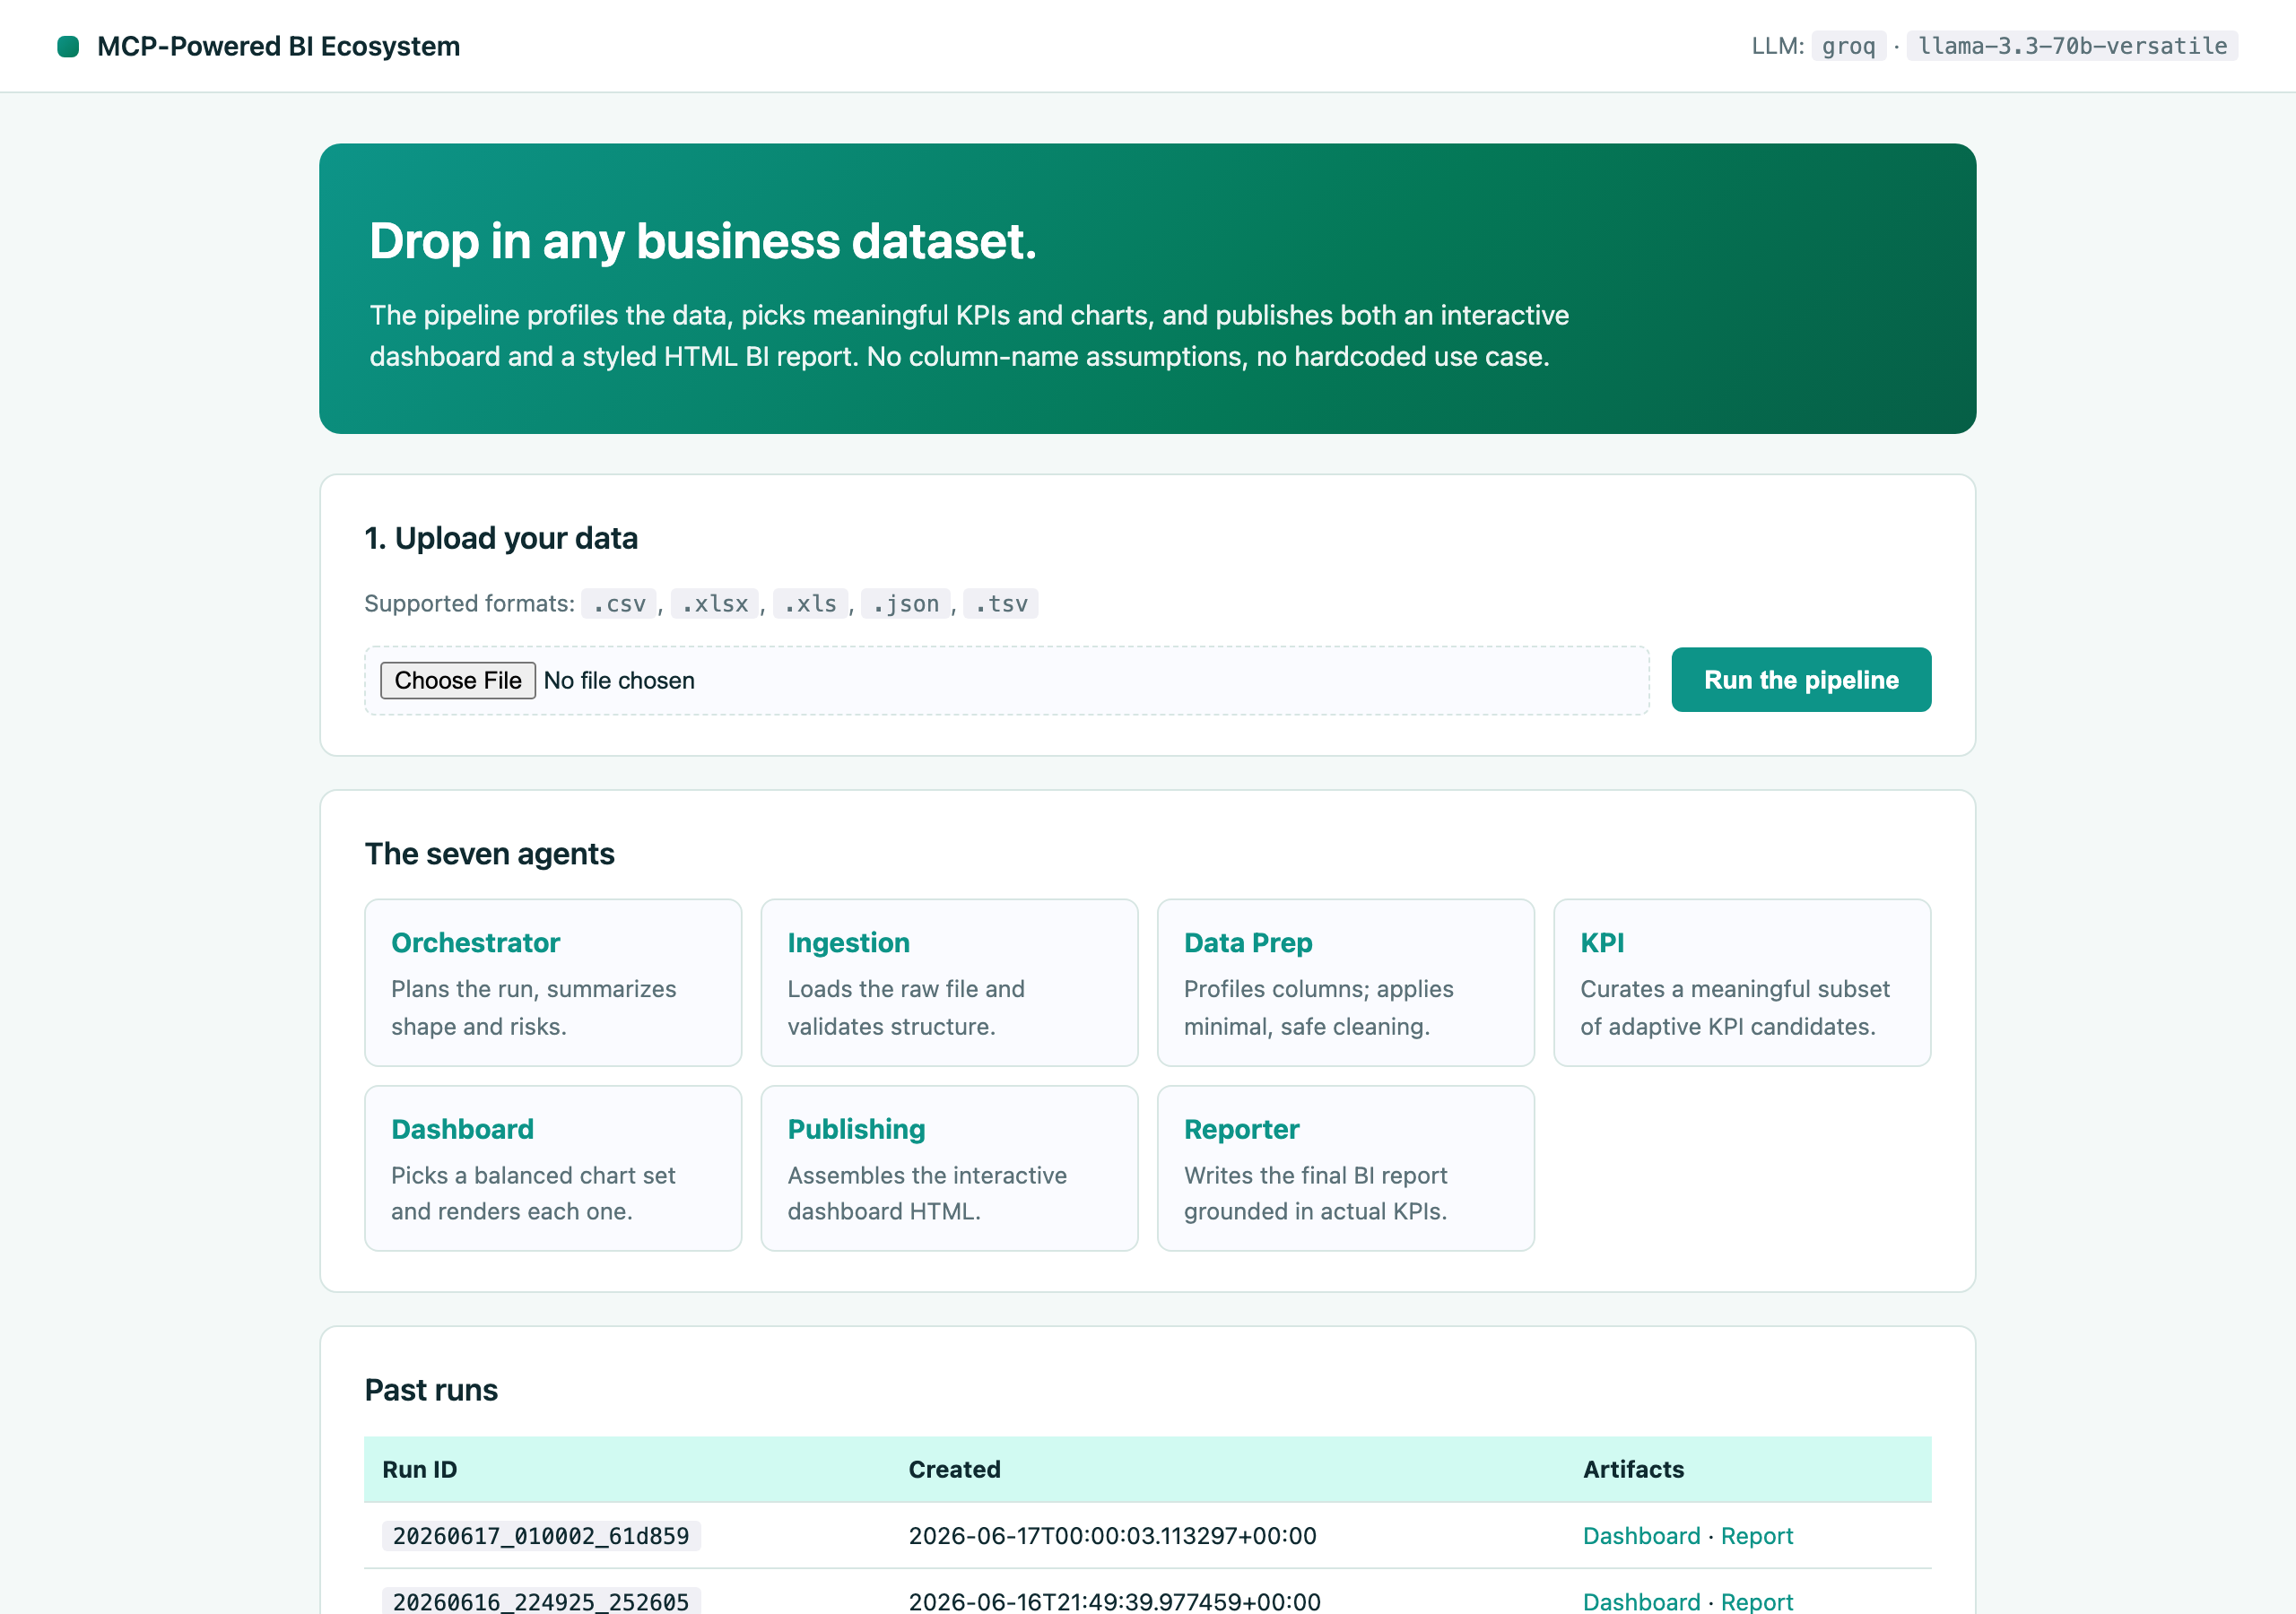
\includegraphics[width=0.86\linewidth]{fig_accueil.png}
\caption{Page d'accueil : téléversement, présentation des agents et historique.}
\label{fig:accueil}
\end{figure}

Après téléversement, le traitement s'exécute en arrière-plan et l'utilisateur
suit sa \textbf{progression par étape}. La figure~\ref{fig:pipeline} montre la
vue d'exécution : statut de chaque agent, indicateurs de consommation (jetons,
coût estimé, latence) et résultat de la vérification des chiffres.

\begin{figure}[ht]
\centering
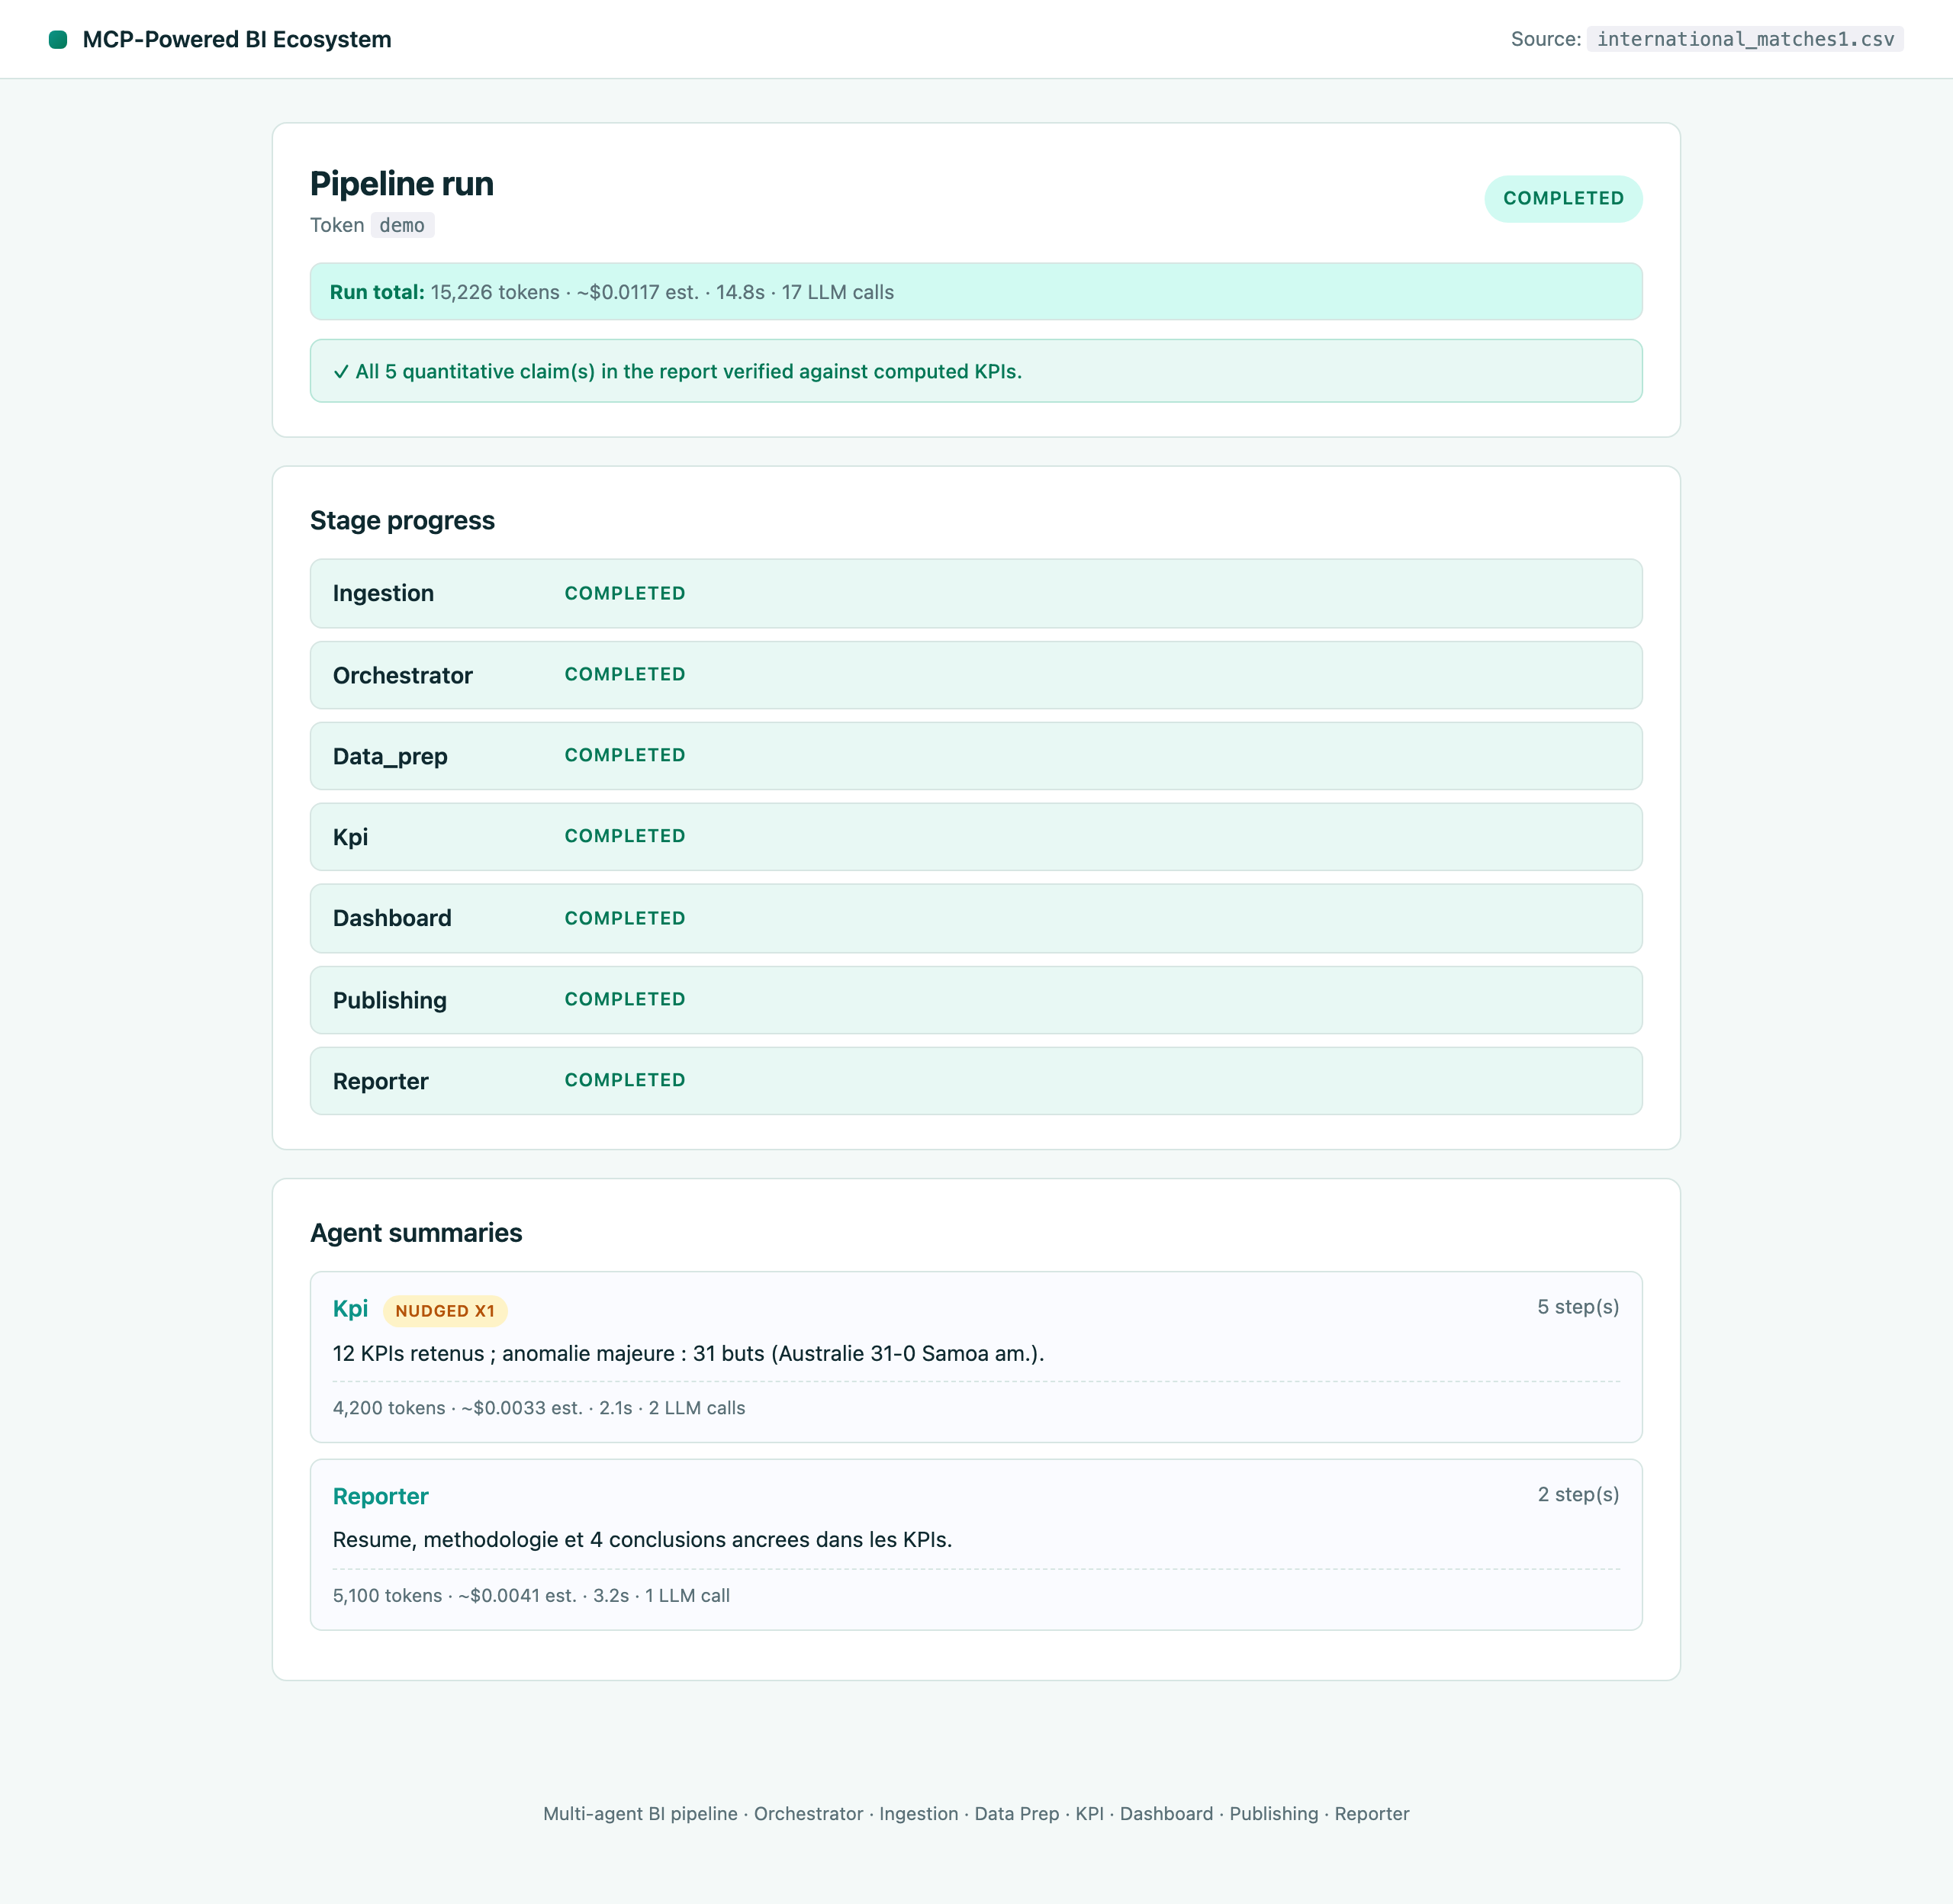
\includegraphics[width=0.74\linewidth]{fig_pipeline.png}
\caption{Suivi en temps réel de l'exécution du pipeline et synthèse des agents.}
\label{fig:pipeline}
\end{figure}

\section{Abstraction des fournisseurs de LLM}
Pour garantir la portabilité, l'accès aux modèles de langage passe par une
\textbf{abstraction} unique (\texttt{src/llm/client.py}) qui masque les
différences entre fournisseurs. Une fabrique sélectionne, selon la
configuration, le client \textbf{Groq} (hébergé, faible latence) ou
\textbf{Ollama} (local, sans clé d'API). Les deux exposent la même méthode
\texttt{chat()} acceptant des outils au format OpenAI et renvoyant un message
normalisé, enrichi de la consommation (jetons) et de la latence. Ce dernier
point alimente le suivi des coûts (section~\ref{sec:couts}).

\begin{lstlisting}[language=Python,caption={Sélection du fournisseur de LLM (\texttt{llm/client.py}).}]
def get_llm_client():
    provider = os.getenv("LLM_PROVIDER", "groq").lower()
    if provider == "groq":
        return GroqClient(api_key=os.getenv("GROQ_API_KEY"),
                          model=os.getenv("GROQ_MODEL"))
    if provider == "ollama":
        return OllamaClient(host=os.getenv("OLLAMA_HOST"),
                            model=os.getenv("OLLAMA_MODEL"))
    raise RuntimeError(f"Fournisseur inconnu : {provider!r}")
\end{lstlisting}

Cette conception applique le principe d'\textbf{inversion de dépendance} : les
agents dépendent d'une interface abstraite (\texttt{LLMClient}) et non d'un
fournisseur concret, ce qui permet d'en changer sans modifier le reste du
code.

\section{Ingestion, validation et profilage adaptatif}
L'agent d'\textbf{Ingestion} charge le fichier (l'extension détermine le
lecteur pandas approprié) puis valide sa structure (doublons, colonnes
entièrement vides, nombre de lignes). Le profilage, cœur de la généralité du
système, attribue à chaque colonne un rôle sémantique. L'extrait~\ref{lst:profiler}
illustre l'inférence du rôle pour les colonnes textuelles, où la détection
\textbf{géographique} est testée en priorité.

\begin{lstlisting}[language=Python,caption={Inférence de rôle pour une colonne textuelle (\texttt{profiler.py}).},label=lst:profiler]
# 4. Chaine de caracteres / objet
else:
    # La geographie est testee en premier et prime sur la cardinalite :
    # une colonne de noms de pays est geographique meme tres cardinale.
    if _looks_like_geo(s, geo_match_threshold):
        role = ColumnRole.GEO
    elif _looks_like_identifier(str(col), card, row_count, is_numeric=False):
        role = ColumnRole.IDENTIFIER
    elif card <= categorical_max_cardinality:
        role = ColumnRole.DIMENSION
    elif card > categorical_max_cardinality and card / max(row_count, 1) > 0.5:
        role = ColumnRole.TEXT
    else:
        role = ColumnRole.HIGH_CARD_DIM
\end{lstlisting}

La détection géographique compare les valeurs distinctes de la colonne à un
référentiel d'environ 250 noms de pays ; si une fraction suffisante
correspond (seuil paramétrable, 0,6 par défaut), la colonne devient une
dimension géographique exploitable par la carte.

\section{Calcul adaptatif des indicateurs (KPI)}
L'agent \textbf{KPI} récupère une liste généreuse de KPIs candidats déduits du
profil, en \textbf{cure} un sous-ensemble pertinent (jugement métier du LLM),
puis les calcule de façon déterministe. Chaque KPI est décrit par une
spécification JSON (identifiant, titre, type, mesure, agrégation, format), ce
qui permet un calcul générique. La figure~\ref{fig:kpis} montre les cartes
d'indicateurs telles qu'elles apparaissent dans le rapport.

\begin{figure}[ht]
\centering
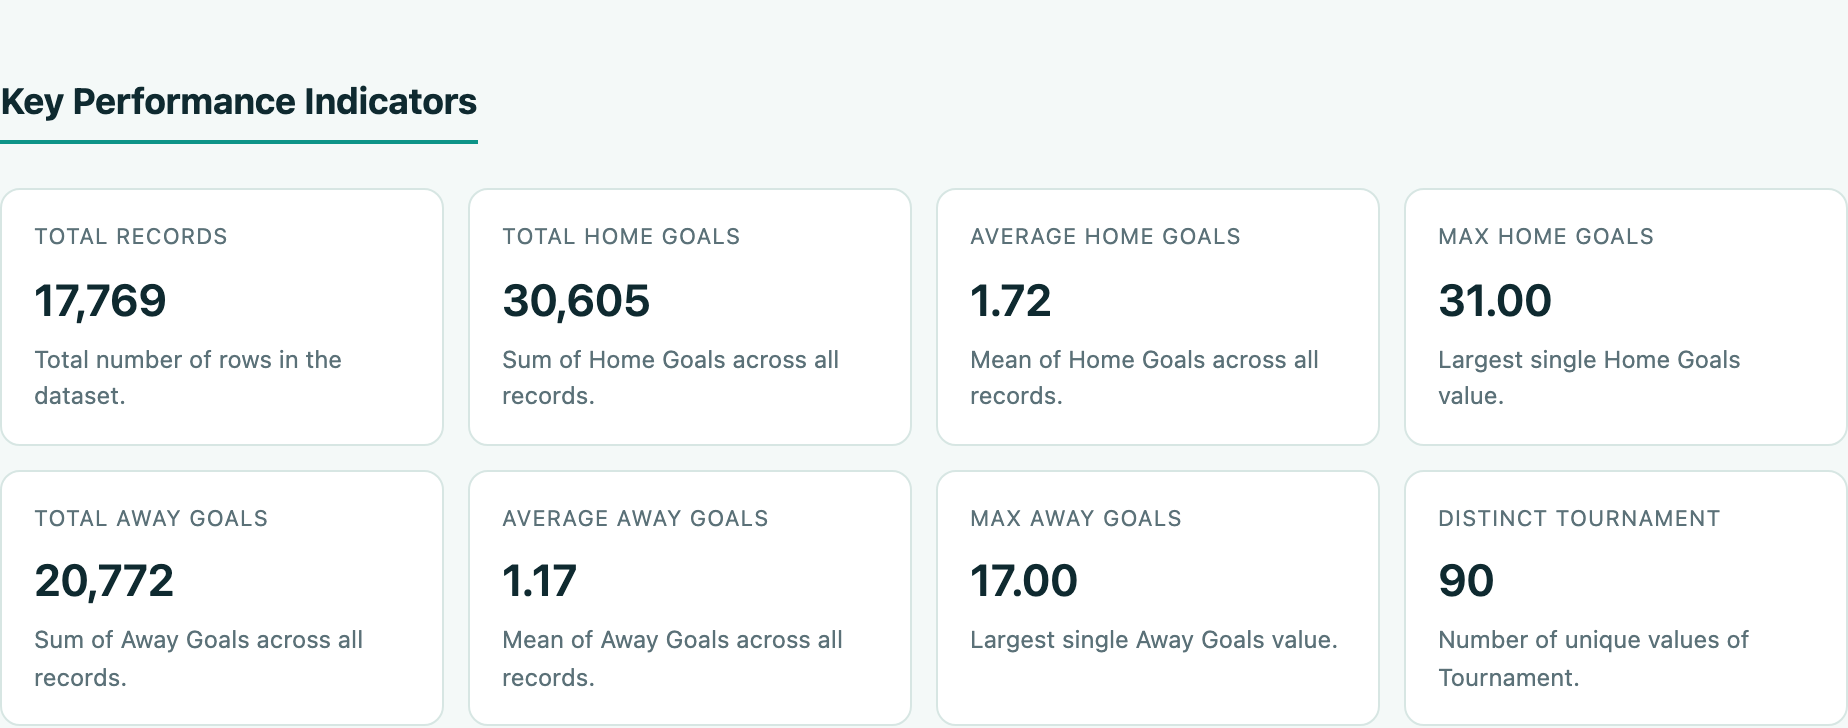
\includegraphics[width=0.92\linewidth]{fig_rapport_kpis.png}
\caption{Indicateurs clés calculés automatiquement (extrait du rapport).}
\label{fig:kpis}
\end{figure}

\section{Visualisations et tableau de bord}
L'agent \textbf{Dashboard} sélectionne un ensemble \textbf{équilibré} de
graphiques (tendance, comparaison, distribution, composition, carte) et les
construit avec Plotly. Le moteur choisit automatiquement le type de graphique
selon les rôles des colonnes. La figure~\ref{fig:dashboard} présente le haut
du tableau de bord généré.

\begin{figure}[ht]
\centering
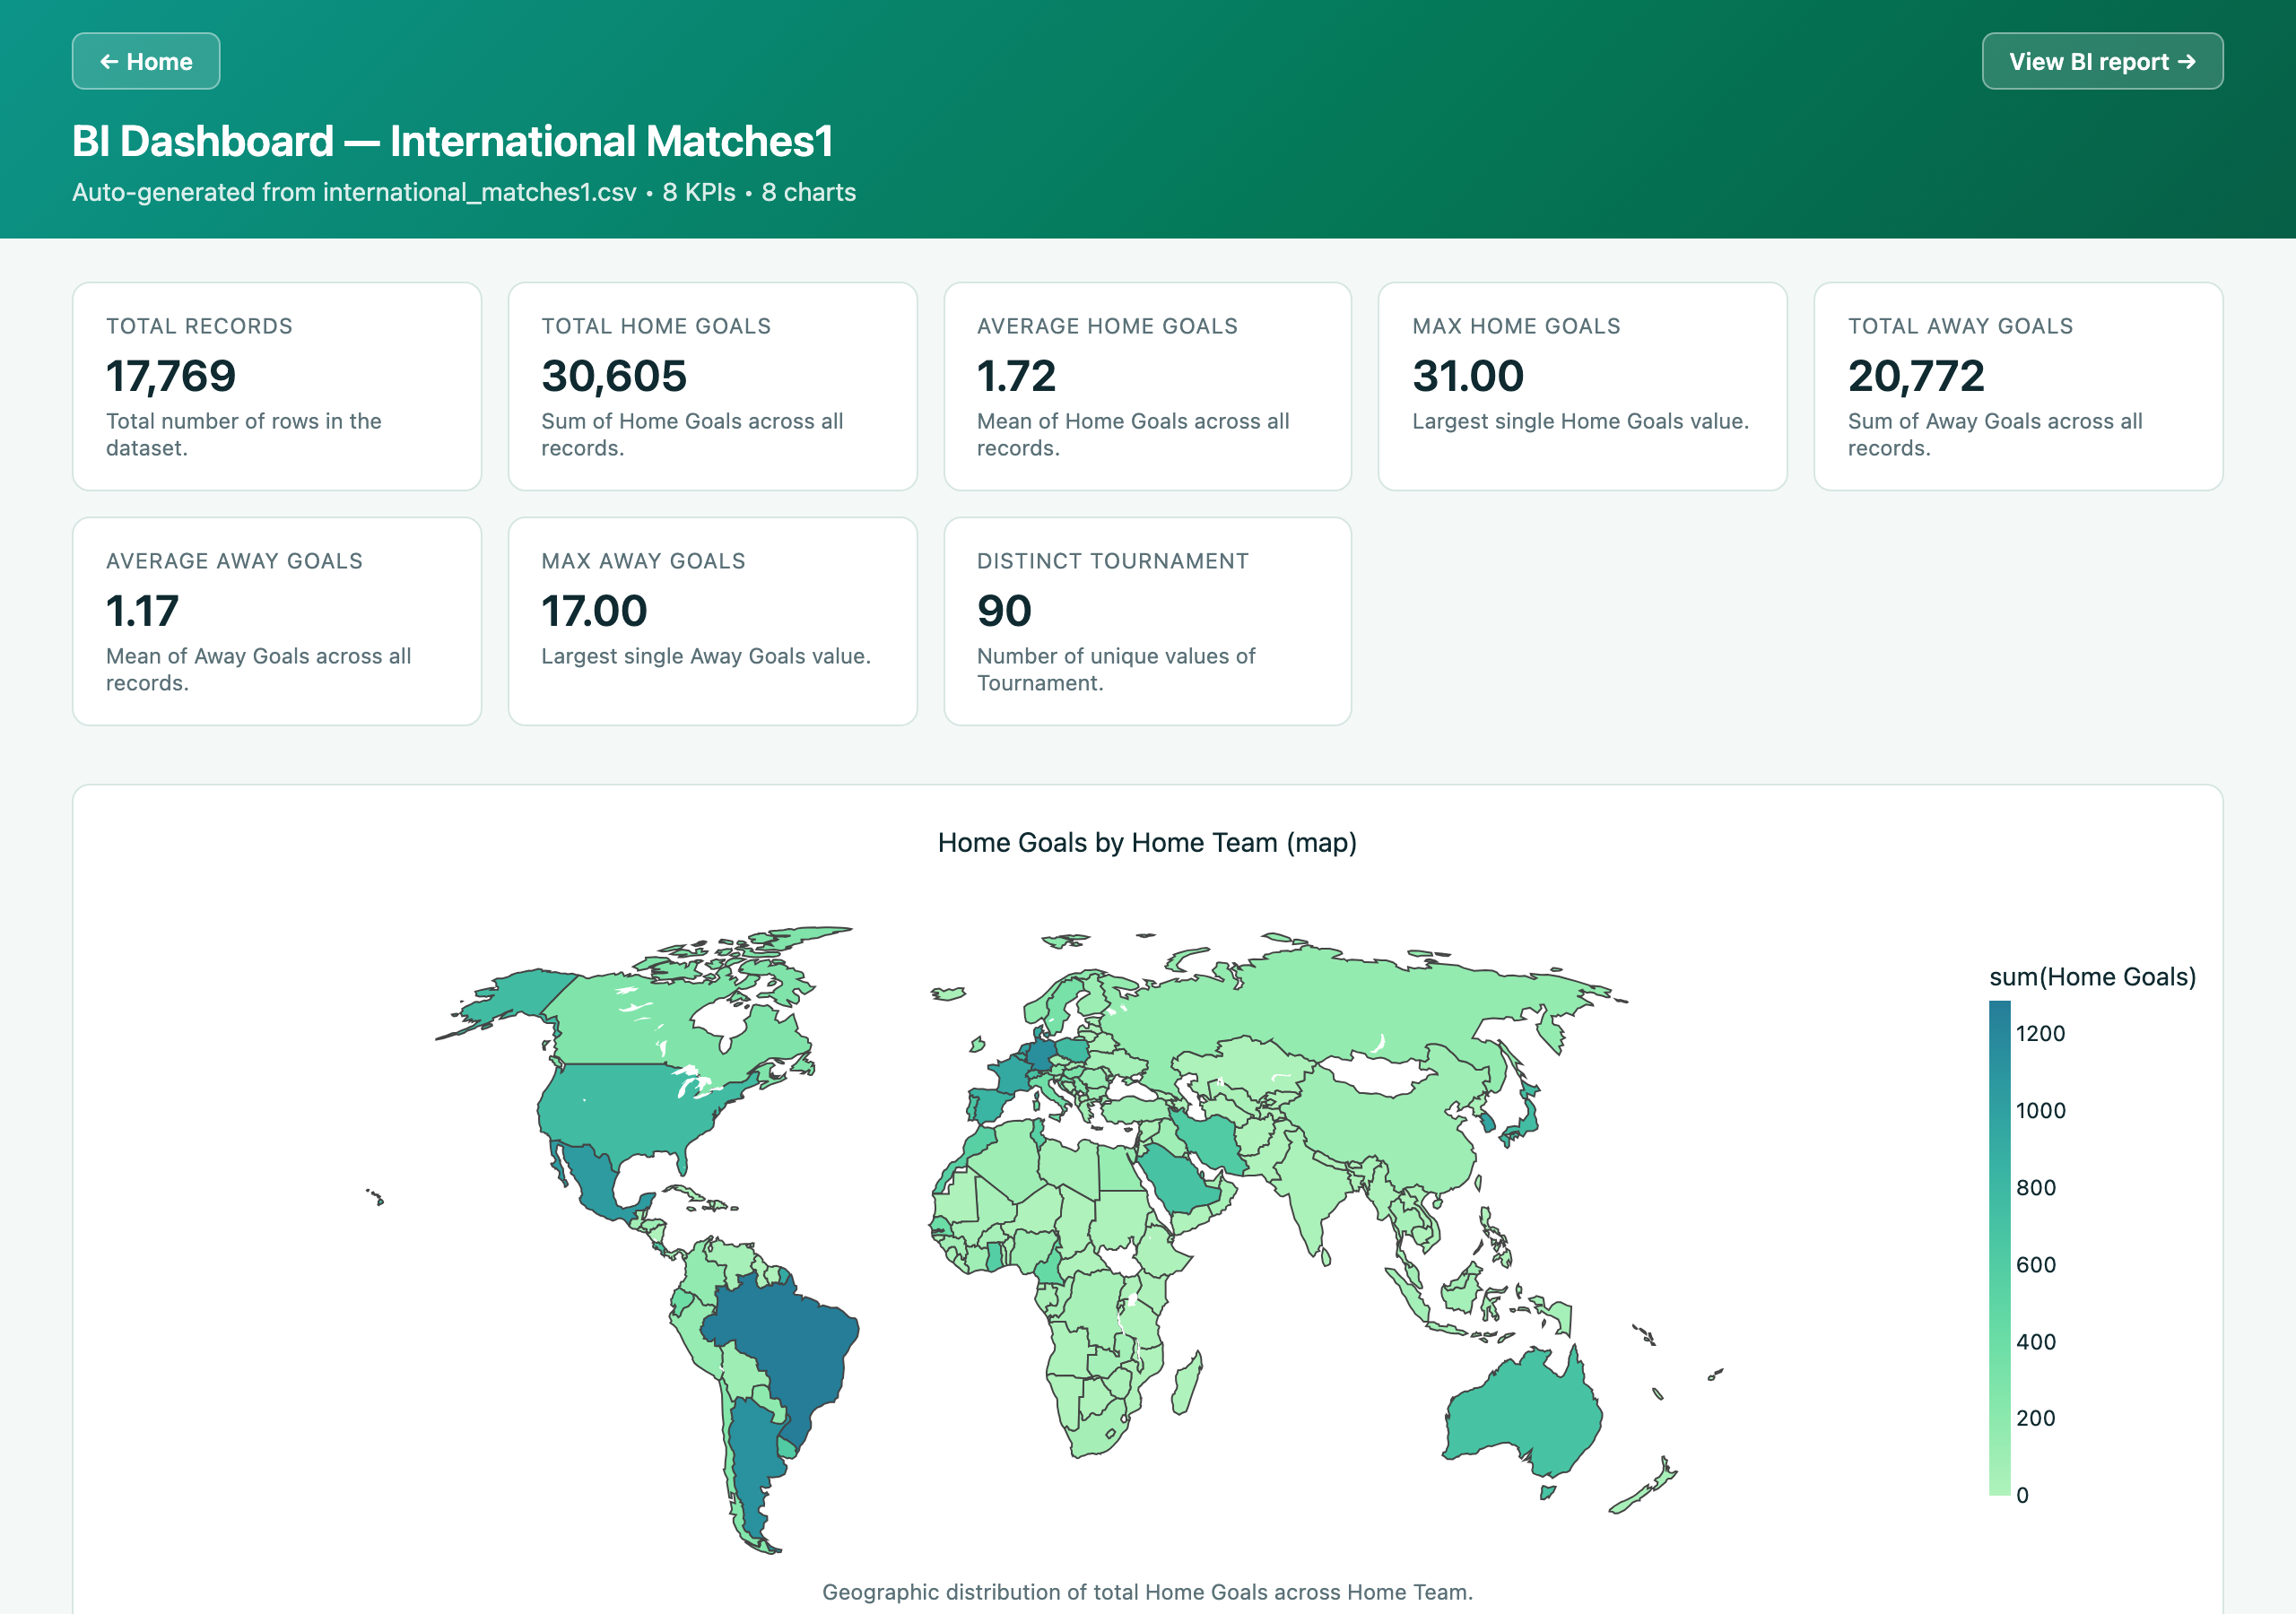
\includegraphics[width=0.9\linewidth]{fig_dashboard.png}
\caption{Tableau de bord interactif : navigation, indicateurs et début de la carte.}
\label{fig:dashboard}
\end{figure}

\subsection{La carte géographique (choroplèthe)}
Lorsqu'une colonne géographique est détectée, le moteur produit une
\textbf{carte choroplèthe} mondiale agrégeant une mesure par pays. La
figure~\ref{fig:carte} en donne un exemple : la distribution des buts à
domicile cumulés par pays.

\begin{figure}[ht]
\centering
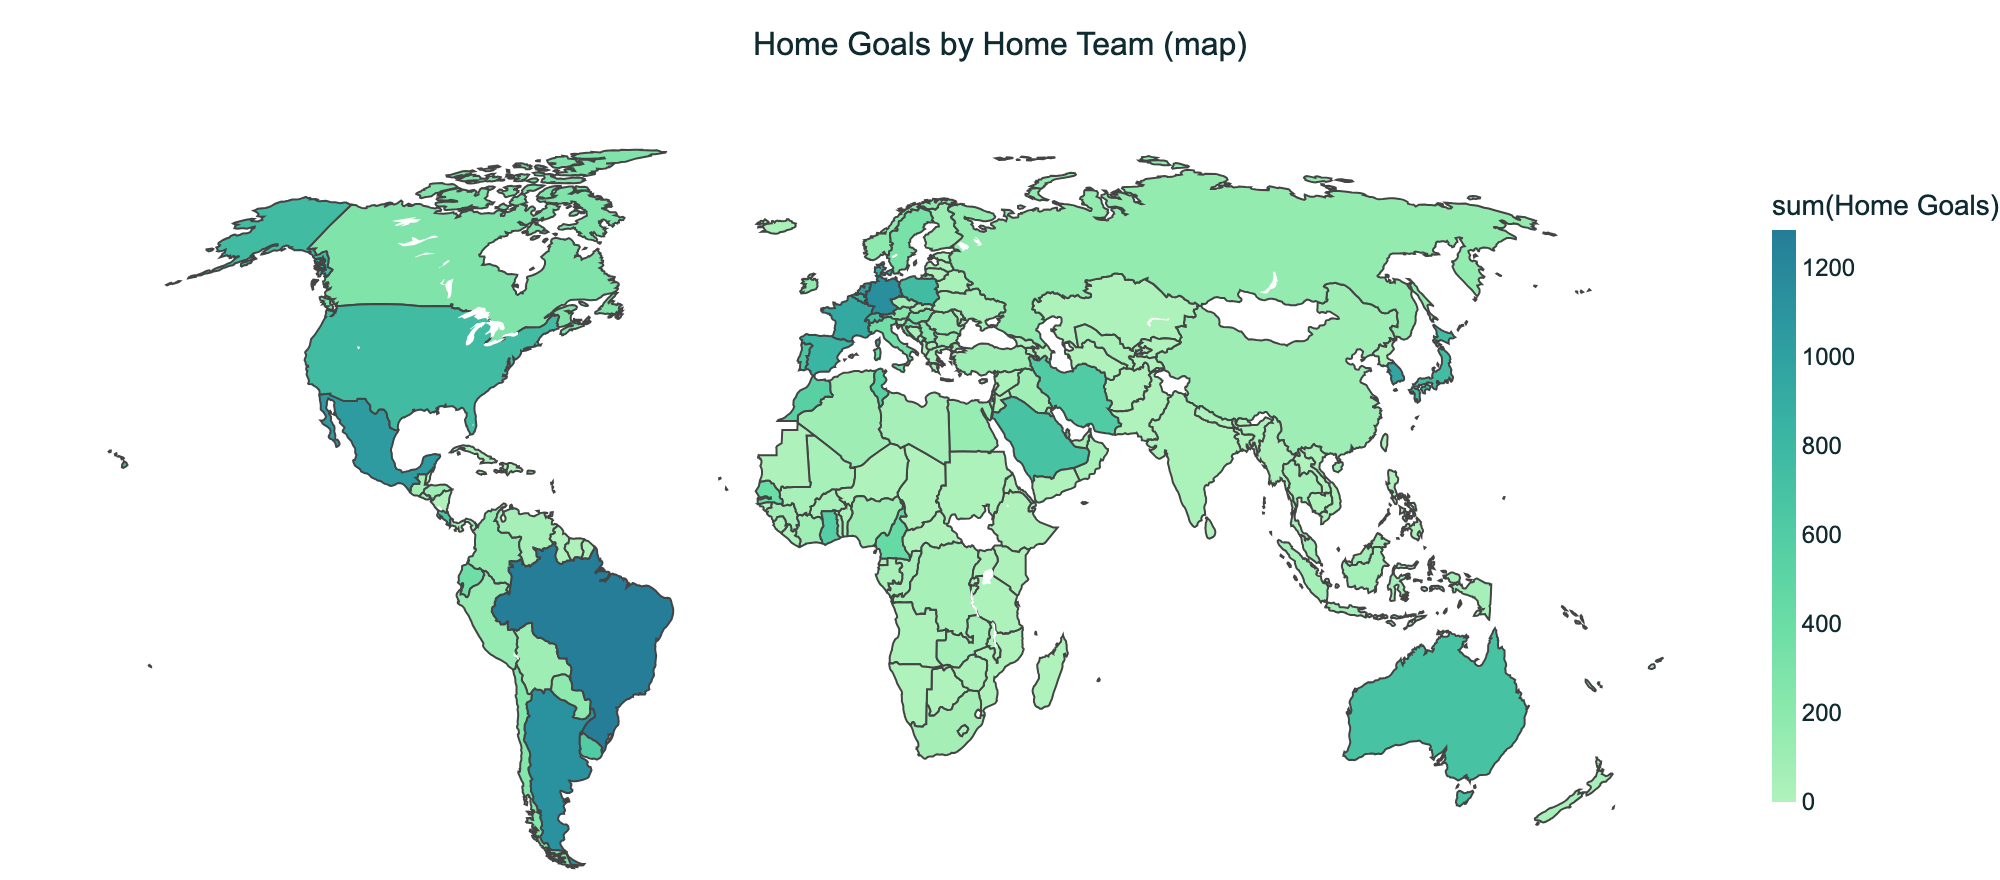
\includegraphics[width=0.92\linewidth]{fig_carte.png}
\caption{Carte choroplèthe : buts à domicile cumulés par pays.}
\label{fig:carte}
\end{figure}

\subsection{Tendances temporelles}
Lorsqu'une colonne de type date est présente, le moteur génère des séries
temporelles, en agrégeant automatiquement par période adaptée au volume de
points. Les figures~\ref{fig:serieH} et~\ref{fig:serieA} illustrent
l'évolution des buts à domicile et à l'extérieur.

\begin{figure}[ht]
\centering
\begin{minipage}{0.49\linewidth}\centering
  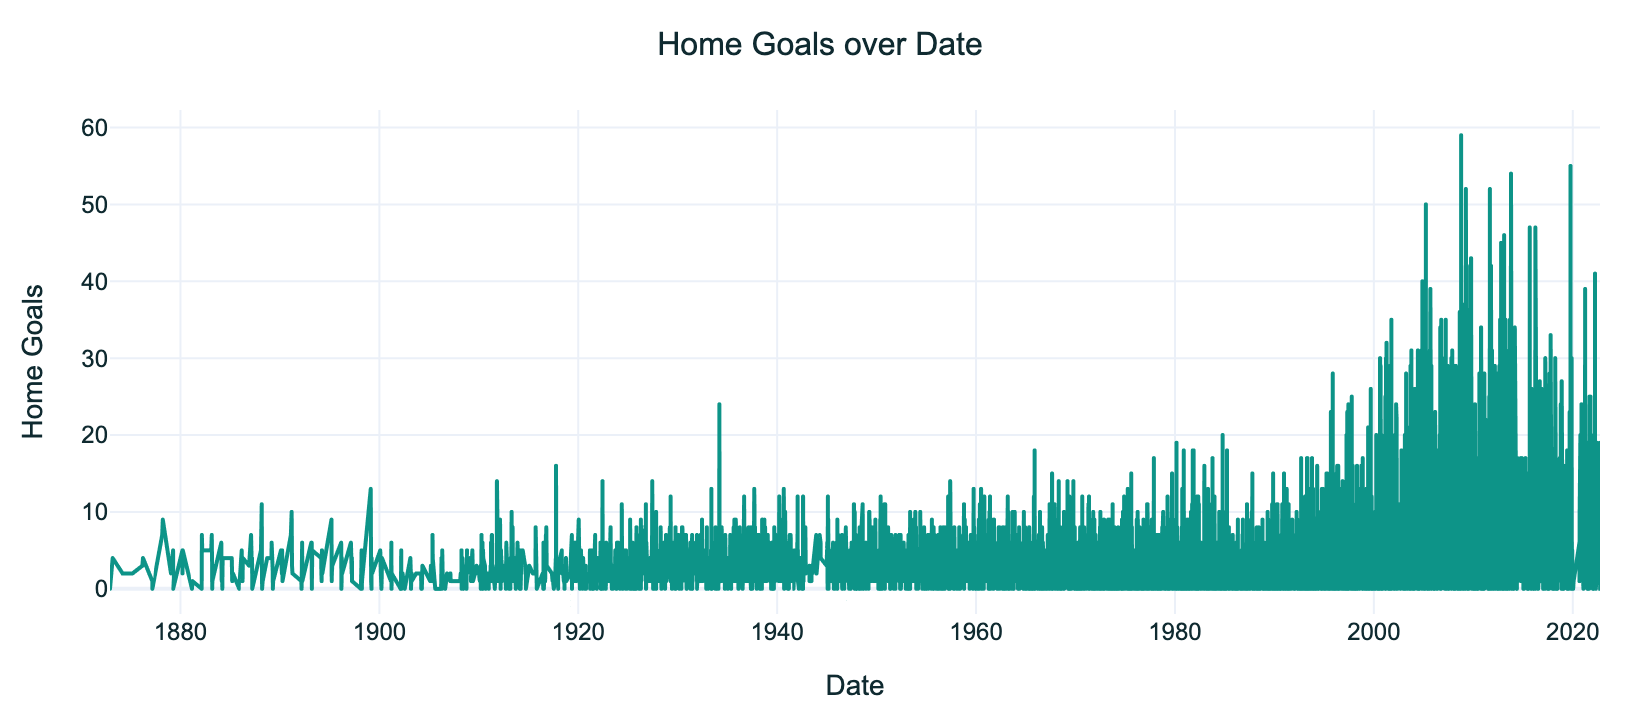
\includegraphics[width=\linewidth]{fig_serie_home.png}
  \caption{Buts à domicile au fil du temps.}
  \label{fig:serieH}
\end{minipage}\hfill
\begin{minipage}{0.49\linewidth}\centering
  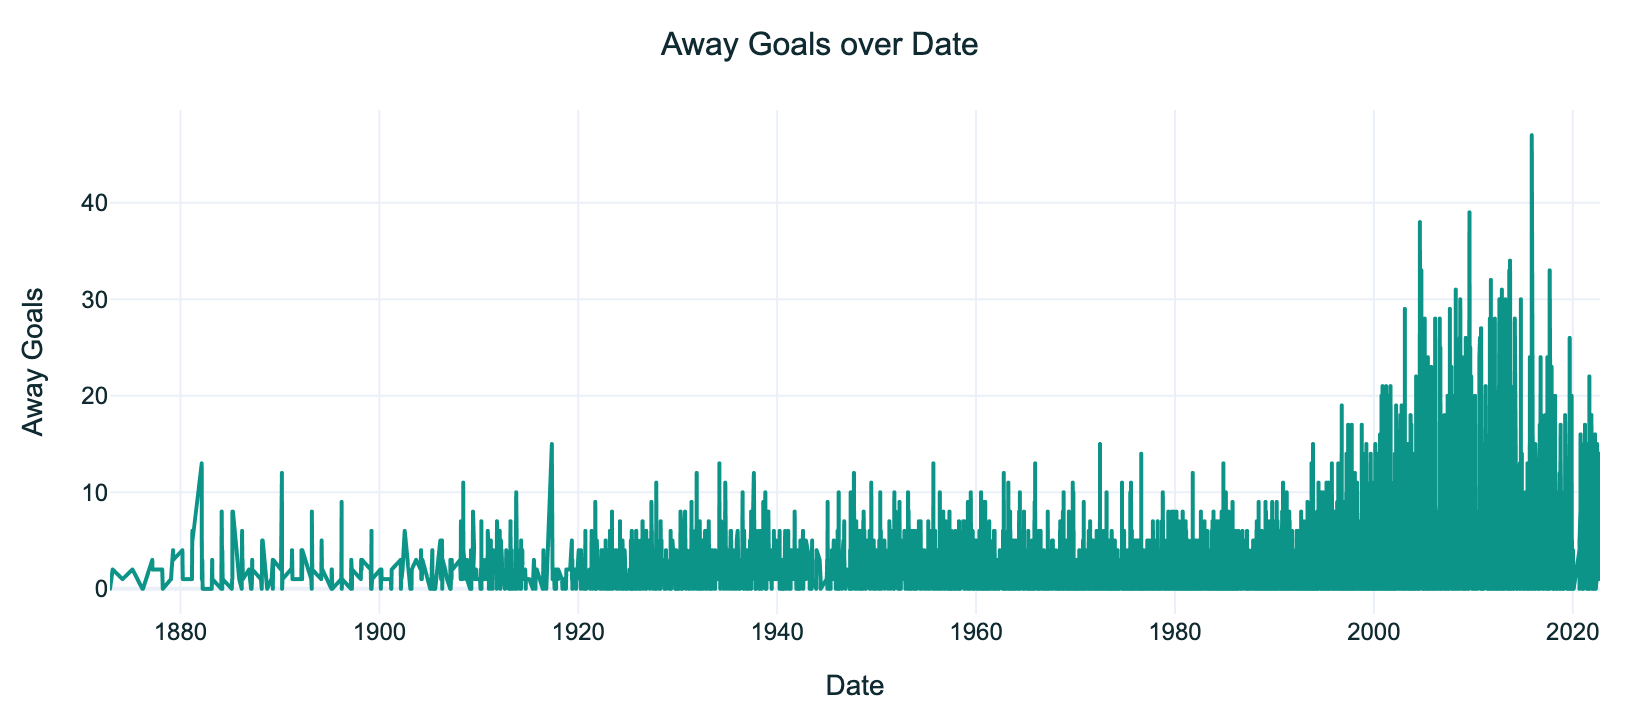
\includegraphics[width=\linewidth]{fig_serie_away.png}
  \caption{Buts à l'extérieur au fil du temps.}
  \label{fig:serieA}
\end{minipage}
\end{figure}

\subsection{Comparaisons et distributions}
Les graphiques en barres top-N classent les valeurs d'une dimension par mesure
(figures~\ref{fig:topT} et~\ref{fig:topE}), tandis que les
\textbf{histogrammes} révèlent la distribution des mesures
(figure~\ref{fig:distribution}), faisant apparaître l'asymétrie typique du
nombre de buts (forte concentration sur les faibles valeurs, longue traîne).

\begin{figure}[ht]
\centering
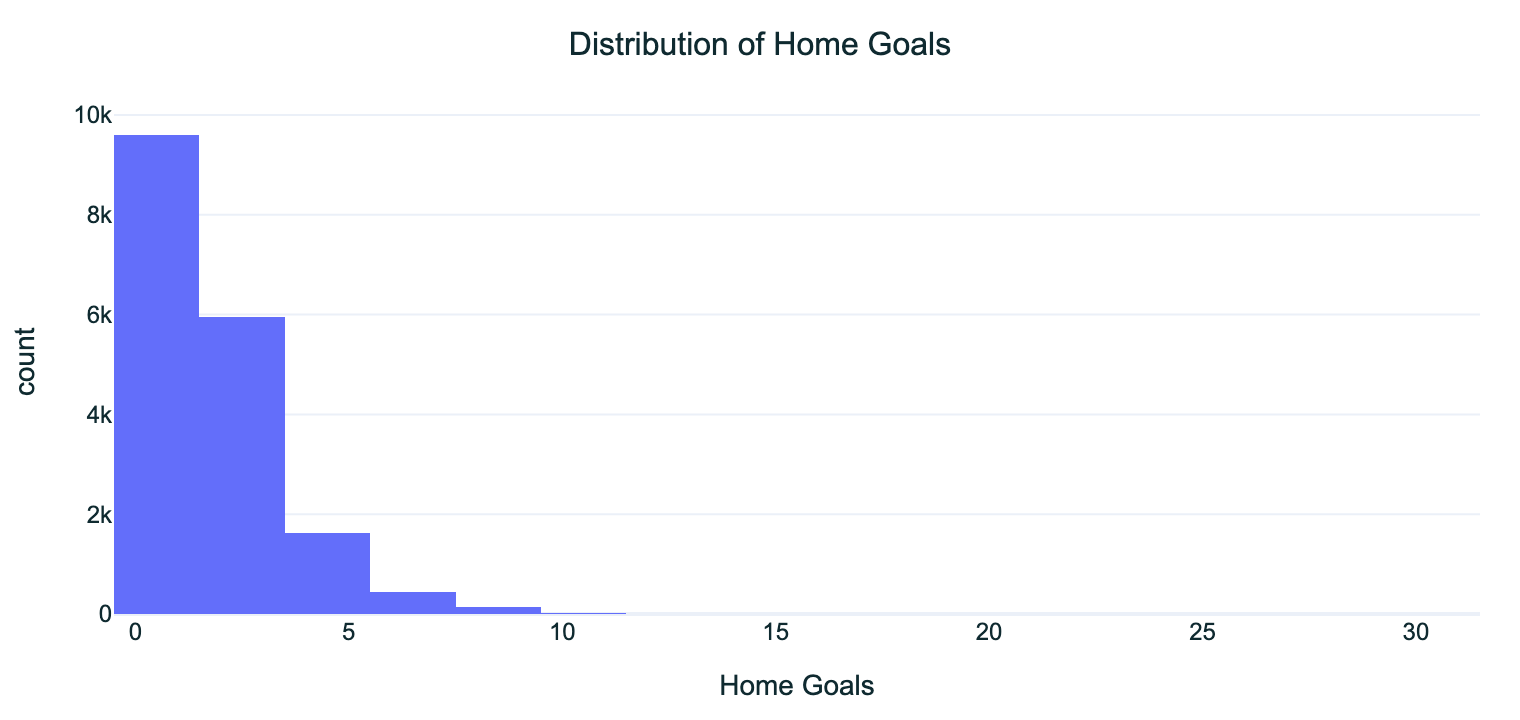
\includegraphics[width=0.62\linewidth]{fig_distribution.png}
\caption{Distribution des buts à domicile (histogramme).}
\label{fig:distribution}
\end{figure}

\begin{figure}[ht]
\centering
\begin{minipage}{0.49\linewidth}\centering
  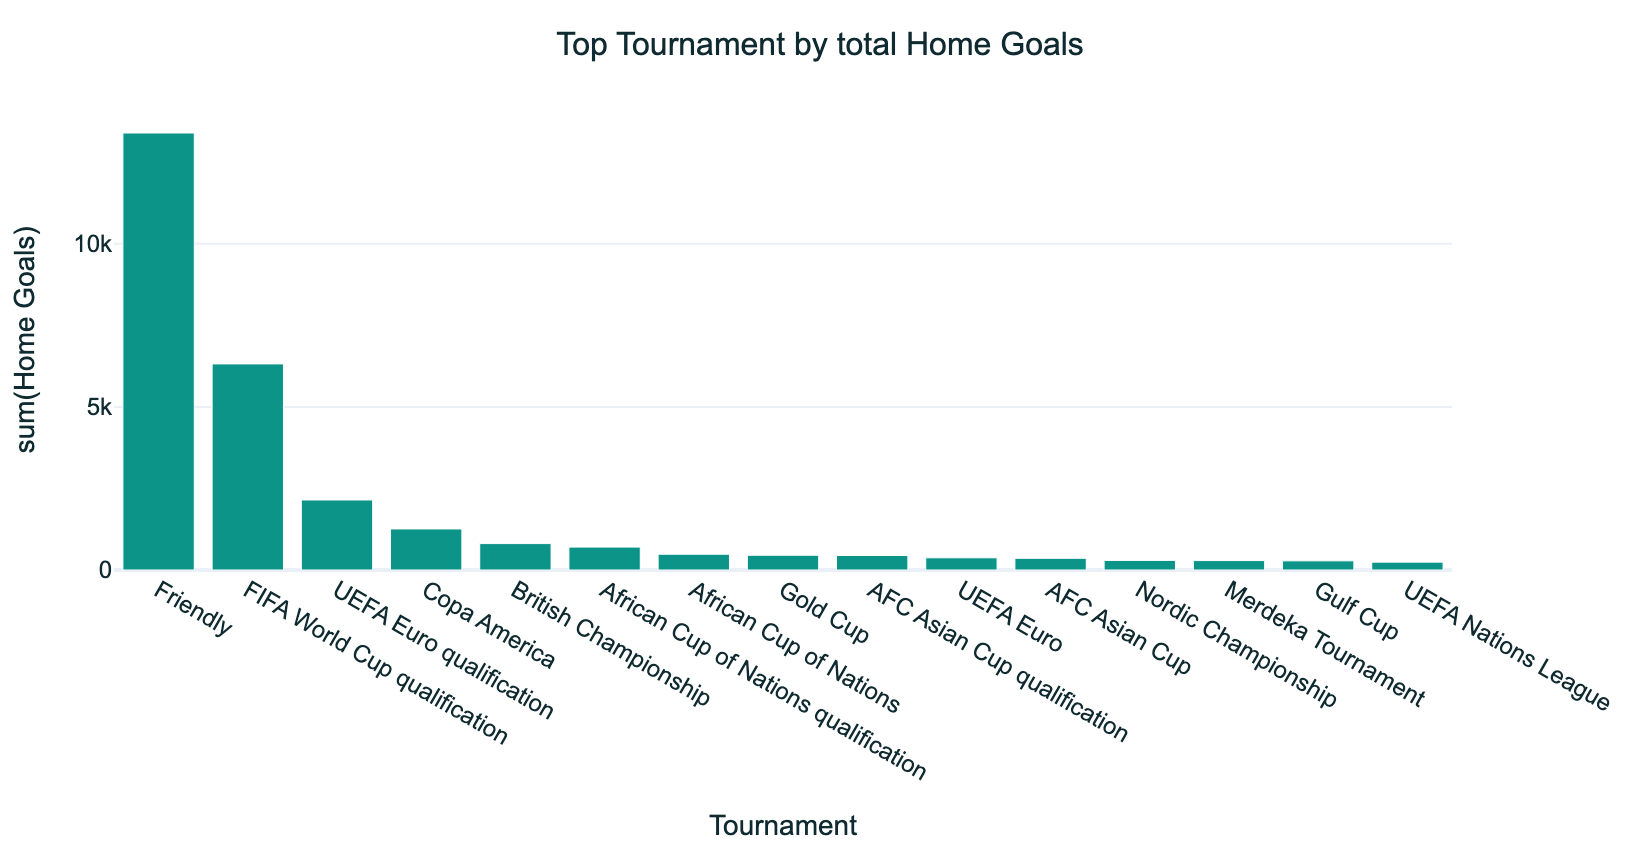
\includegraphics[width=\linewidth]{fig_top_tournois.png}
  \caption{Top tournois par buts à domicile.}
  \label{fig:topT}
\end{minipage}\hfill
\begin{minipage}{0.49\linewidth}\centering
  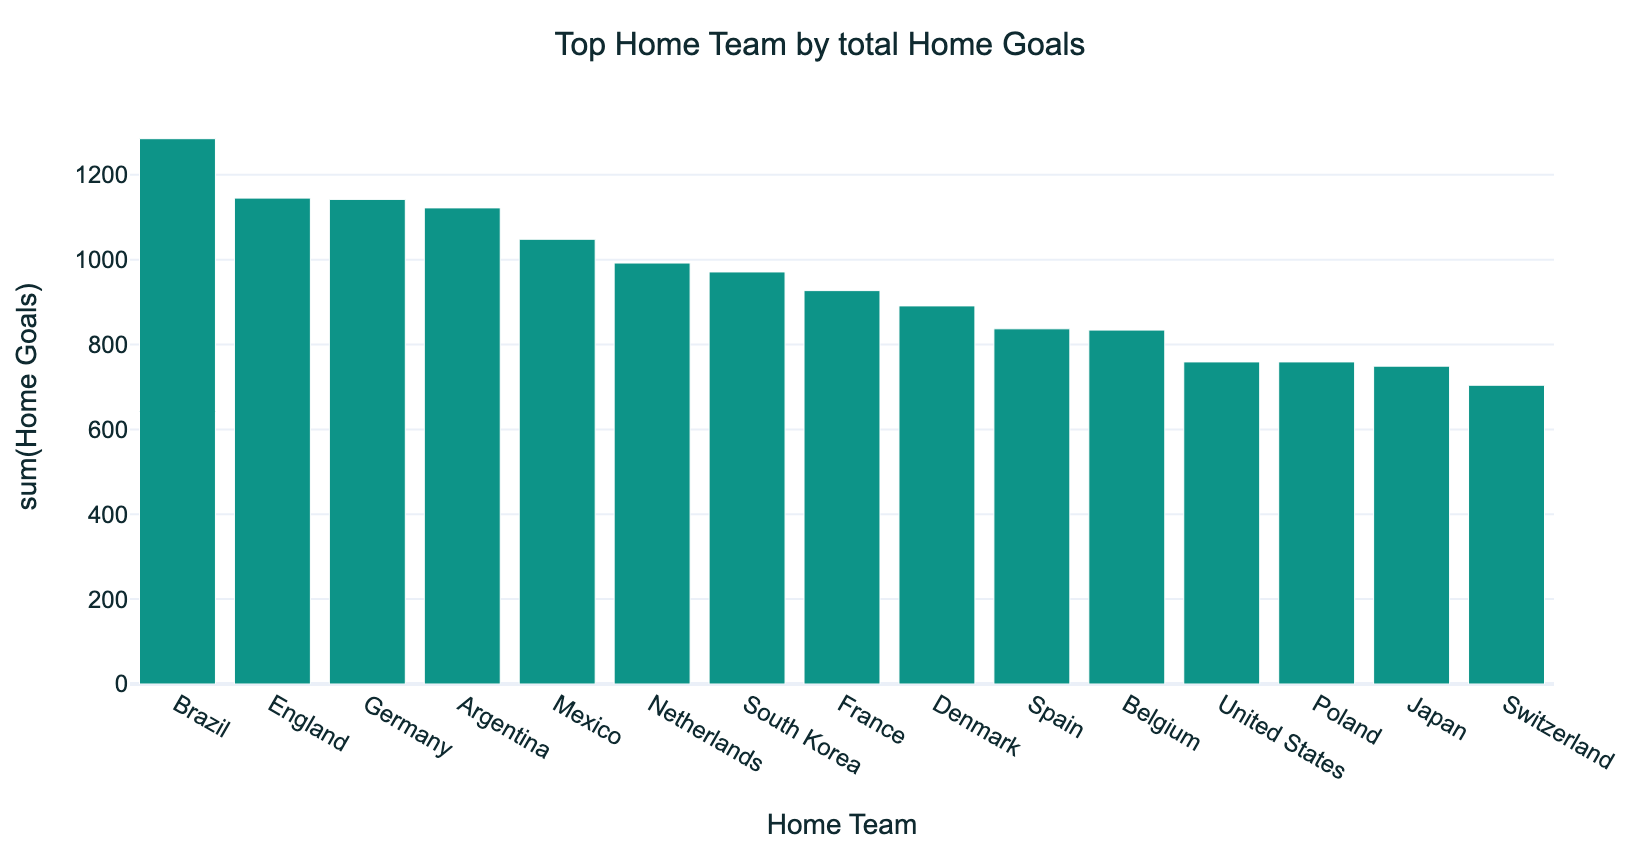
\includegraphics[width=\linewidth]{fig_top_equipes.png}
  \caption{Top équipes par buts à domicile.}
  \label{fig:topE}
\end{minipage}
\end{figure}

\section{Analyses avancées : anomalies et segments}
L'agent KPI enrichit l'analyse de deux familles d'insights, implémentés dans
\texttt{src/core/insights.py}.

\subsection{Détection d'anomalies}
La détection repose sur un \textbf{score z modifié} fondé sur l'écart absolu
médian (MAD), robuste aux valeurs extrêmes que l'on cherche précisément à
isoler (extrait~\ref{lst:anomalies}).

\begin{lstlisting}[language=Python,caption={Score z modifié robuste (\texttt{insights.py}).},label=lst:anomalies]
def _modified_z(values):
    median = np.median(values)
    mad = np.median(np.abs(values - median))
    if mad == 0:
        return None  # pas de dispersion : repli sur l'ecart interquartile
    return 0.6745 * (values - median) / mad
\end{lstlisting}

Toute valeur dont le score dépasse un seuil (3,5 par défaut) est signalée. La
figure~\ref{fig:anomalies} montre la restitution dans le rapport.

\begin{figure}[ht]
\centering
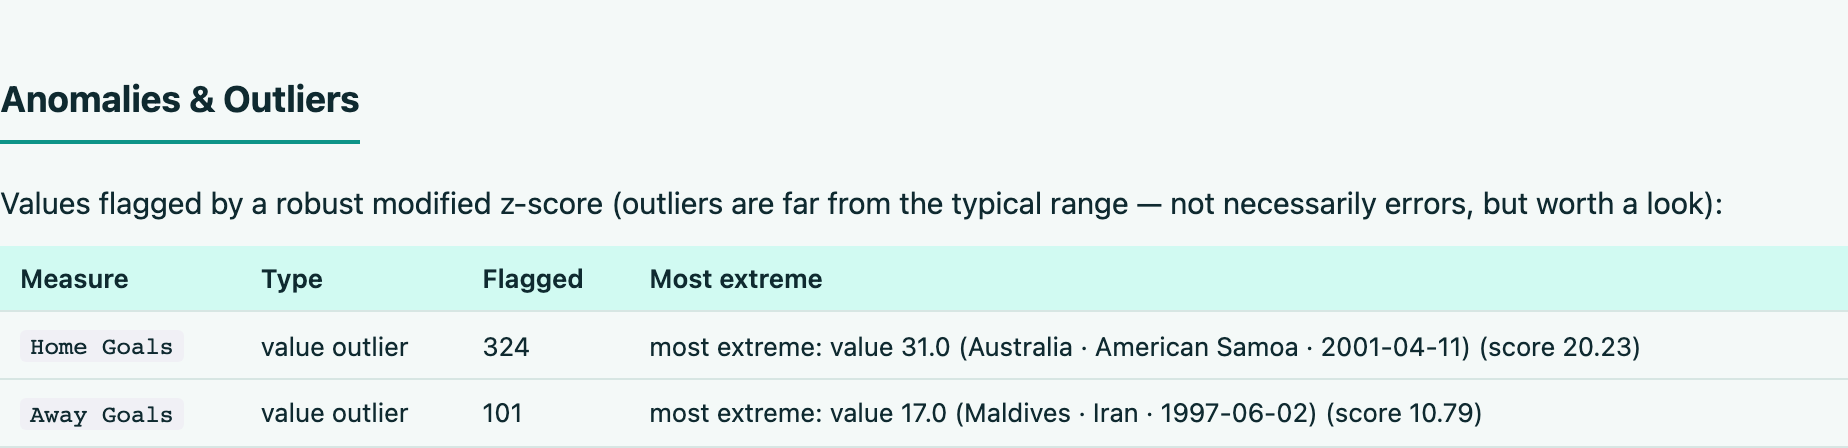
\includegraphics[width=0.92\linewidth]{fig_rapport_anomalies.png}
\caption{Section « Anomalies » du rapport : valeurs aberrantes et exemple le plus extrême.}
\label{fig:anomalies}
\end{figure}

\subsection{Comparaison de segments}
Pour chaque dimension de faible cardinalité et chaque mesure, le moteur
compare les moyennes par groupe et retient les écarts les plus marqués
(figure~\ref{fig:segments}). Cette analyse met par exemple en évidence
l'avantage du terrain dans l'étude de cas.

\begin{figure}[ht]
\centering
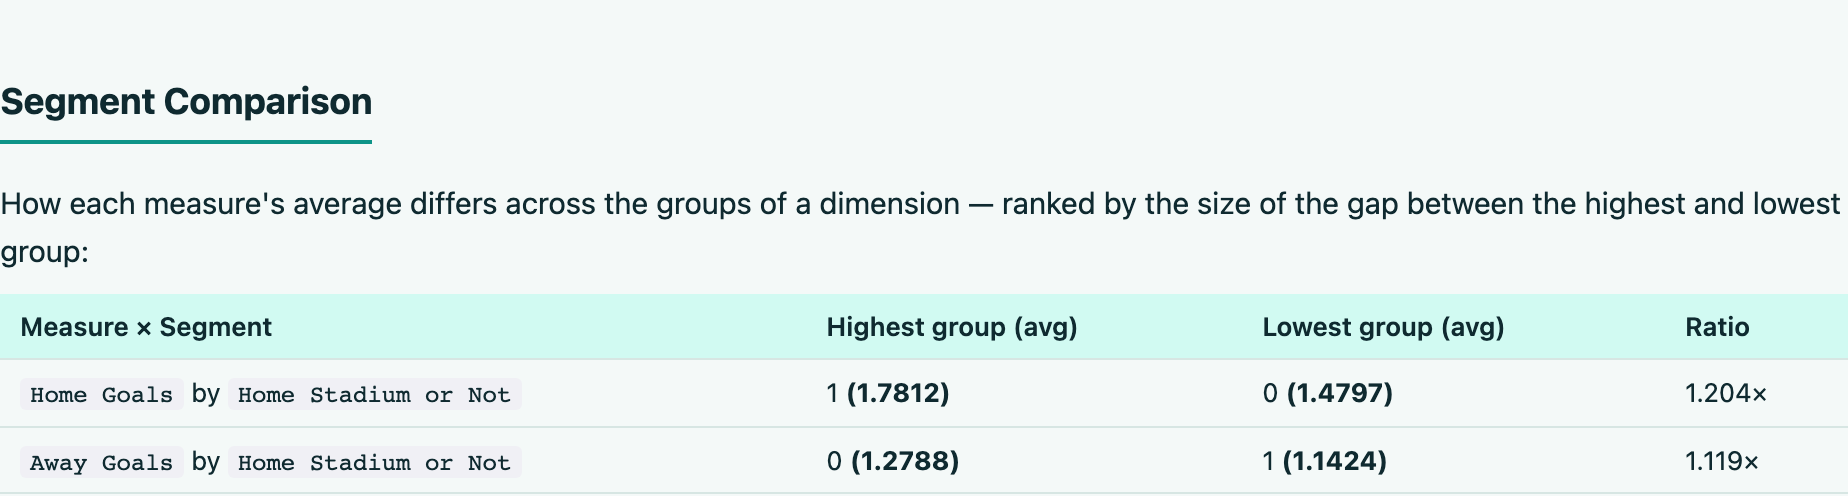
\includegraphics[width=0.92\linewidth]{fig_rapport_segments.png}
\caption{Section « Comparaison de segments » du rapport.}
\label{fig:segments}
\end{figure}

\section{Orchestration et filets de sécurité}
Le pipeline (\texttt{src/pipeline.py}) exécute les sept agents dans un ordre
déterministe. Comme un agent peut, en pratique, omettre un appel d'outil, des
\textbf{filets de sécurité} déterministes vérifient après chaque étape que les
sorties attendues existent et, le cas échéant, invoquent eux-mêmes les outils
manquants sous les permissions du rôle concerné. L'extrait~\ref{lst:fallback}
illustre ce dispositif pour l'étape KPI.

\begin{lstlisting}[language=Python,caption={Filet de sécurité de l'étape KPI (\texttt{pipeline.py}).},label=lst:fallback]
elif stage == "kpi":
    if not store.get("kpis"):
        # ... calcul des KPIs si l'agent les a omis ...
        _safe("kpi", "compute_kpis", {"kpi_ids": top_ids})
    # Les insights sont independants des KPIs : on garantit chacun.
    if store.get("anomalies") is None:
        _safe("kpi", "detect_anomalies", {})
    if store.get("segments") is None:
        _safe("kpi", "compare_segments", {})
\end{lstlisting}

Ce mécanisme garantit qu'une exécution produit \textbf{toujours} des livrables
complets, même en cas de défaillance d'un agent — le moteur déterministe
devenant le filet de dernier recours.

\section{Publication des livrables}
L'agent de \textbf{Publication} assemble le tableau de bord interactif
(\texttt{dashboard.html}) et fige l'état complet de l'exécution
(\texttt{state.json}). L'agent \textbf{Reporter} produit ensuite le
\textbf{rapport décisionnel} (\texttt{report.html}), structuré en sections :
résumé, source des données, méthodologie, indicateurs, tableau de bord,
conclusions, anomalies, comparaison de segments. Le rapport est exportable en
\textbf{PDF} (impression navigateur) et en \textbf{HTML} autonome ; chaque
graphique est exportable en image. La figure~\ref{fig:entete} montre l'en-tête
du rapport avec sa barre d'actions et de navigation.

\begin{figure}[ht]
\centering

\includegraphics[width=0.92\linewidth]{fig_rapport_entete.png}
\caption{En-tête du rapport : navigation (Accueil, Dashboard) et export (PDF, HTML).}
\label{fig:entete}
\end{figure}

\section{Fiabilité : véracité des chiffres et suivi des coûts}

\subsection{Vérification des chiffres du rapport}
Pour contrer les hallucinations, chaque nombre cité dans les conclusions du
rapport est \textbf{vérifié} face à l'ensemble des nombres réellement calculés
(valeurs des KPIs, statistiques du profil, comptages, corrélations, valeurs
d'anomalies, moyennes de segments), avec une tolérance absorbant les arrondis.
Le rapport affiche alors un verdict : \emph{vérifié}, \emph{partiel} ou
\emph{non vérifié}. La figure~\ref{fig:findings} montre le badge de
vérification au-dessus des conclusions.

\begin{figure}[ht]
\centering
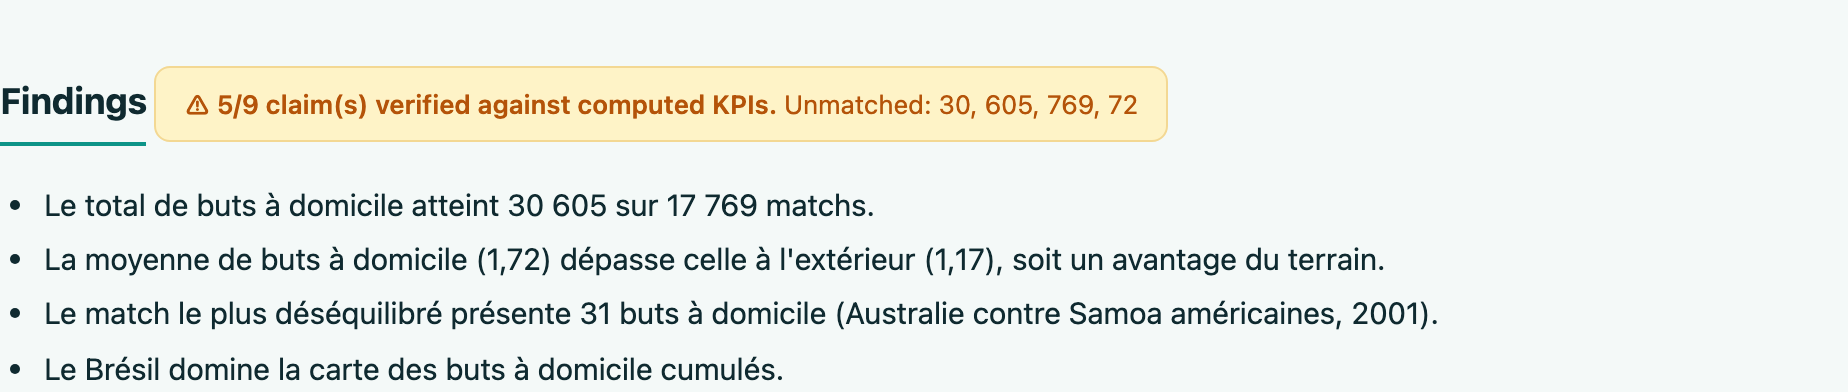
\includegraphics[width=0.92\linewidth]{fig_rapport_findings.png}
\caption{Conclusions du rapport avec le badge de vérification des chiffres.}
\label{fig:findings}
\end{figure}

\subsection{Suivi de la consommation}
\label{sec:couts}
Le client LLM mesure, pour chaque appel, le nombre de jetons (entrée/sortie)
et la latence ; le pipeline agrège ces mesures par agent et par exécution, et
estime un coût à partir de prix paramétrables. Ces indicateurs sont restitués
dans la vue d'exécution (figure~\ref{fig:pipeline}), assurant l'observabilité
du système.

\callout{Synthèse du chapitre}{Le système combine un moteur déterministe
généraliste (profilage, KPIs, graphiques, carte, insights) et des agents qui
curent et narrent. Les filets de sécurité garantissent des livrables complets,
la vérification des chiffres assure la véracité, et le suivi des coûts apporte
l'observabilité. Le chapitre suivant évalue l'ensemble.}

\chapter{Tests, résultats et étude de cas}
\label{chap:tests}

\callout{En bref}{Ce chapitre présente la stratégie de validation du système,
les résultats des tests automatisés, puis une étude de cas approfondie sur un
jeu de 17 769 matchs internationaux de football, avant une discussion des
apports et des limites.}

\section{Stratégie de tests}
La qualité du système repose sur une suite de \textbf{22 tests automatisés}
(exécutés avec \texttt{pytest}), couvrant à la fois le moteur déterministe et
la logique d'orchestration. Deux principes ont guidé cette stratégie :
\begin{itemize}
  \item \textbf{tester sans LLM} : le cœur déterministe est validé
        indépendamment de tout fournisseur de modèle, ce qui rend les tests
        rapides et reproductibles ;
  \item \textbf{simuler les défaillances d'agents} : un client LLM
        « fictif » permet de vérifier que les filets de sécurité produisent
        des livrables complets même lorsque les agents n'appellent aucun outil.
\end{itemize}

Le tableau~\ref{tab:tests} récapitule la couverture par module.

\begin{table}[ht]
\centering\small
\caption{Couverture des tests automatisés.}
\label{tab:tests}
\begin{tabularx}{\linewidth}{@{}Yc@{}}
\toprule
\textbf{Domaine testé} & \textbf{Nb. de tests} \\
\midrule
Profilage des rôles de colonnes & 1 \\
Suggestion et calcul des KPIs & 1 \\
Suggestion et construction des graphiques & 1 \\
Assemblage du tableau de bord HTML & 1 \\
Permissions du serveur MCP (refus hors périmètre) & 1 \\
Vérification des chiffres (\texttt{validation.py}) & 7 \\
Relance avec incitation (\textit{retry-with-nudge}) & 2 \\
Détection géographique \& carte choroplèthe & 3 \\
Détection d'anomalies & 2 \\
Comparaison de segments & 2 \\
Extraction numérique robuste & 1 \\
\midrule
\textbf{Total} & \textbf{22} \\
\bottomrule
\end{tabularx}
\end{table}

L'ensemble des 22 tests est au vert. Au-delà des tests unitaires, des
\textbf{exécutions de bout en bout} sur des jeux de données réels valident
l'intégration complète (du téléversement aux artefacts produits).

\section{Étude de cas : matchs internationaux de football}

\subsection{Présentation du jeu de données}
Pour valider l'approche généraliste, nous avons soumis au système un jeu de
données de \textbf{17 769 matchs internationaux de football} disputés entre
\textbf{1872 et 2024}. Aucune configuration spécifique n'a été fournie : le
système a découvert seul la structure des données. Le profilage automatique a
identifié :
\begin{itemize}
  \item 2 \textbf{mesures} : buts à domicile (\textit{Home Goals}) et à
        l'extérieur (\textit{Away Goals}) ;
  \item 2 colonnes \textbf{géographiques} : équipe à domicile et à
        l'extérieur (reconnues comme des pays) ;
  \item 1 colonne \textbf{date}, et plusieurs \textbf{dimensions}
        (tournoi, ville, stade neutre ou non) ;
  \item 90 tournois, 214 équipes à domicile et 218 à l'extérieur.
\end{itemize}

La figure~\ref{fig:source} montre la section « source des données » du rapport
généré, incluant le schéma détecté et le résultat de la validation.

\begin{figure}[ht]
\centering
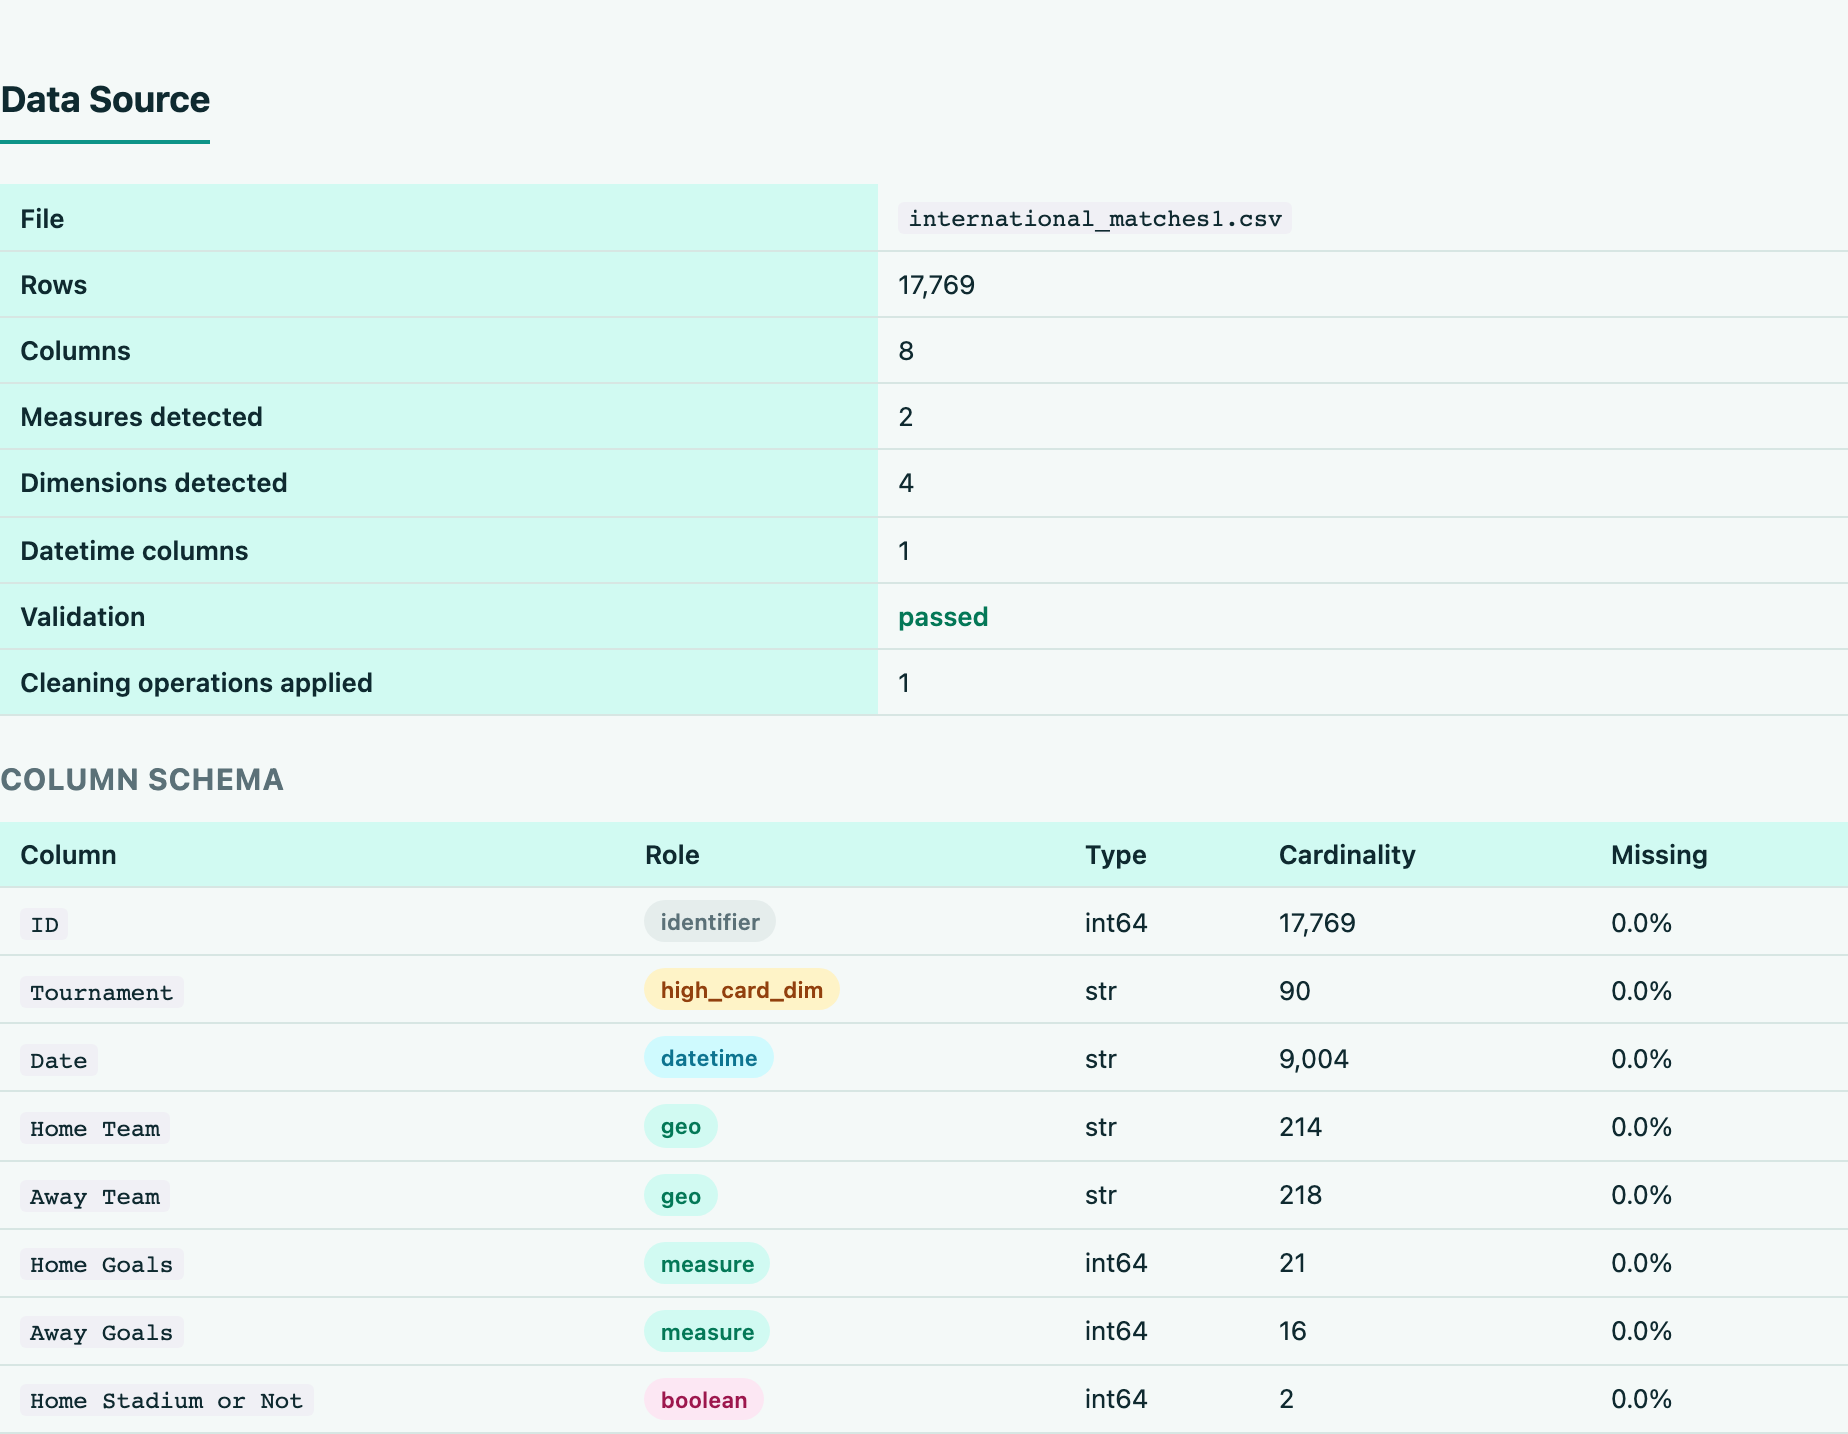
\includegraphics[width=0.92\linewidth]{fig_rapport_source.png}
\caption{Section « source des données » : schéma détecté automatiquement et validation.}
\label{fig:source}
\end{figure}

\subsection{Résultats : indicateurs et tableau de bord}
Le système a produit automatiquement un tableau de bord complet et un rapport.
Parmi les indicateurs calculés :
\begin{itemize}
  \item un total de \textbf{30 605 buts à domicile} sur l'ensemble des matchs ;
  \item une moyenne de \textbf{1,72} but à domicile contre \textbf{1,17} à
        l'extérieur ;
  \item un maximum de \textbf{31 buts} marqués en un seul match.
\end{itemize}

Le tableau~\ref{tab:resultats} récapitule les principaux indicateurs produits
automatiquement par le système pour ce jeu de données.

\begin{table}[ht]
\centering\small
\caption{Indicateurs clés calculés pour l'étude de cas.}
\label{tab:resultats}
\begin{tabularx}{\linewidth}{@{}Yr@{}}
\toprule
\textbf{Indicateur} & \textbf{Valeur} \\
\midrule
Nombre total de matchs & 17\,769 \\
Total des buts à domicile & 30\,605 \\
Moyenne de buts à domicile & 1,72 \\
Moyenne de buts à l'extérieur & 1,17 \\
Maximum de buts en un match & 31 \\
Tournois distincts & 90 \\
Équipes à domicile distinctes & 214 \\
Équipes à l'extérieur distinctes & 218 \\
\bottomrule
\end{tabularx}
\end{table}

La \textbf{carte choroplèthe} (figure~\ref{fig:carte}, chapitre précédent)
révèle d'un coup d'œil la domination du \textbf{Brésil} en buts cumulés à
domicile, suivi des grandes nations européennes et sud-américaines. Les
\textbf{séries temporelles} (figures~\ref{fig:serieH} et~\ref{fig:serieA})
montrent une nette intensification du nombre de buts après l'an 2000, reflet de
la multiplication des rencontres internationales.

\subsection{Résultats : anomalies détectées}
La détection d'anomalies a automatiquement isolé des matchs au score
exceptionnel. Le plus extrême correspond au match historique
\textbf{Australie 31--0 Samoa américaines} (2001), record du monde de buts
inscrits en un match international, correctement identifié comme valeur
aberrante (score~z très élevé). Côté extérieur, le match \textbf{Maldives
0--17 Iran} (1997) ressort également. Ce résultat illustre la capacité du
système à faire remonter, sans aucune connaissance métier préalable, des
événements réellement remarquables.

\subsection{Résultats : avantage du terrain}
La comparaison de segments a mis en évidence un phénomène bien connu des
analystes du football : l'\textbf{avantage du terrain}. En segmentant selon le
caractère « à domicile ou non » du stade, le système a mesuré une moyenne de
buts supérieure pour l'équipe jouant chez elle (1,78 contre 1,48), confirmant
quantitativement cet effet — là encore, de manière entièrement automatique.

\subsection{Véracité du rapport}
Enfin, le mécanisme de vérification a confirmé que \textbf{l'intégralité des
chiffres} cités dans les conclusions du rapport correspondait aux indicateurs
réellement calculés (verdict « vérifié », figure~\ref{fig:findings} du
chapitre précédent), démontrant l'efficacité du garde-fou anti-hallucination.

\section{Discussion}

\subsection{Apports}
L'étude de cas confirme les promesses de l'approche :
\begin{itemize}
  \item \textbf{généralité} : un jeu de données sportif, jamais anticipé, est
        analysé sans aucune configuration ;
  \item \textbf{pertinence} : les indicateurs, la carte et les insights
        produits sont immédiatement exploitables ;
  \item \textbf{fiabilité} : les chiffres sont exacts et vérifiés, et les
        livrables toujours complets grâce aux filets de sécurité ;
  \item \textbf{rapidité} : l'analyse complète est produite en quelques
        secondes, contre des heures de travail manuel.
\end{itemize}

\subsection{Limites}
Plusieurs limites subsistent :
\begin{itemize}
  \item la détection géographique repose sur des noms de pays en anglais ;
        certaines entités infranationales (Écosse, Pays de Galles) ne sont pas
        cartographiées par la projection mondiale ;
  \item la qualité de la narration dépend du modèle de langage employé ;
  \item le système traite un fichier à la fois et ne gère pas encore les
        jointures entre sources ;
  \item l'analyse reste descriptive (pas de modélisation prédictive).
\end{itemize}
Ces limites ouvrent directement sur les perspectives présentées en conclusion.

\callout{Synthèse du chapitre}{Les 22 tests valident le cœur du système, et
l'étude de cas sur 17 769 matchs démontre une analyse généraliste, pertinente
et fiable : carte mondiale, détection du match record 31--0, mise en évidence
de l'avantage du terrain, et chiffres intégralement vérifiés.}

\chapter*{Conclusion générale et perspectives}
\addcontentsline{toc}{chapter}{Conclusion générale et perspectives}
\markboth{CONCLUSION GÉNÉRALE}{}

Ce projet de fin d'année a abouti à la conception et à la réalisation de
\textbf{\montitre}, une plateforme de Business Intelligence \textbf{généraliste}
et \textbf{automatisée}. Partant du constat que la chaîne décisionnelle
traditionnelle reste manuelle, coûteuse et spécialisée, nous avons proposé une
architecture originale qui réconcilie la rigueur d'un \textbf{moteur
déterministe} et le discernement d'une \textbf{équipe de sept agents
d'intelligence artificielle}, le tout orchestré par le \textbf{protocole MCP}.

Les objectifs fixés en introduction ont été atteints. Une architecture
multi-agents à contrôle d'accès par rôle a été mise en place, et un moteur
adaptatif profile désormais n'importe quel jeu de données pour en dériver
automatiquement indicateurs, graphiques et insights. Le système produit, à
chaque exécution, un tableau de bord interactif et un rapport décisionnel
(web et PDF) reproductibles, tandis que des mécanismes de fiabilité — filets
de sécurité, vérification des chiffres et suivi des coûts — renforcent la
confiance dans les résultats. L'étude de cas menée sur 17 769 matchs
internationaux a enfin validé l'approche de bout en bout. Au-delà du produit,
ce travail nous a permis de consolider des compétences transversales :
conception logicielle en couches, intégration de modèles de langage et d'outils
via un protocole standard, ingénierie de la fiabilité face à des composants non
déterministes, et communication scientifique.

Plusieurs pistes d'évolution prolongent naturellement ce travail. L'ajout d'un
analyste conversationnel permettrait de poser des questions en langage naturel
et d'obtenir réponses et graphiques à la volée, en réutilisant le registre
d'outils MCP existant. L'ingestion pourrait être étendue à de nouvelles sources
de données — bases SQL, feuilles de calcul en ligne, stockage objet — ainsi
qu'aux jointures multi-sources. Des analyses prédictives, telles que la
prévision de séries temporelles et l'identification de facteurs explicatifs,
compléteraient utilement l'analyse descriptive actuelle. Enfin,
l'industrialisation de la plateforme — conteneurisation, persistance des
exécutions, authentification et déploiement multi-utilisateurs — ouvrirait la
voie à une mise en production.

En définitive, \textbf{\montitre} démontre qu'il est possible d'automatiser la
chaîne décisionnelle complète sans sacrifier la fiabilité, en assignant à
chaque composant — moteur déterministe et agents IA — le rôle où il excelle.
Cette complémentarité nous semble une voie prometteuse pour l'avenir des
outils décisionnels.


% ---- Bibliographie --------------------------------------------------
\bibliographystyle{plain}
\bibliography{references}
\addcontentsline{toc}{chapter}{Bibliographie}

% ---- Annexes --------------------------------------------------------
\appendix
\chapter{Annexes}
\markboth{ANNEXES}{}

\section{Guide d'installation et d'exécution}
Le système requiert Python~3.10 ou supérieur.

\begin{lstlisting}[caption={Installation et lancement.}]
# 1. Environnement virtuel
python -m venv .venv
source .venv/bin/activate        # macOS / Linux

# 2. Dependances
pip install -r requirements.txt

# 3. Configuration (fournisseur de LLM)
cp .env.example .env             # renseigner GROQ_API_KEY, ou LLM_PROVIDER=ollama

# 4. Lancement de l'interface web
uvicorn src.ui.app:app --reload
# -> ouvrir http://127.0.0.1:8000
\end{lstlisting}

Il est aussi possible d'exécuter le pipeline en ligne de commande sur un
fichier, ou de générer le jeu de données d'exemple :

\begin{lstlisting}[caption={Exécutions alternatives.}]
# Pipeline en ligne de commande
python -m src.pipeline data/sample_sales.csv

# Generation d'un jeu de donnees d'exemple
python scripts/generate_sample_data.py --out data/sample_sales.csv
\end{lstlisting}

\section{Extrait : matrice de permissions (\texttt{config.yaml})}
La configuration ci-dessous illustre le contrôle d'accès par rôle appliqué
par le serveur MCP.

\begin{lstlisting}[caption={Définition d'un agent et de ses outils autorisés.}]
agents:
  kpi:
    description: >
      Metriques et insights. Curent et calculent les KPIs, puis
      detectent anomalies et comparaisons de segments.
    tools:
      - profile_dataset
      - suggest_kpis
      - compute_kpis
      - detect_anomalies
      - compare_segments
\end{lstlisting}

\section{Extrait : boucle d'appel d'outils d'un agent}
\begin{lstlisting}[language=Python,caption={Cœur de la boucle agentique (\texttt{agents/base.py}).}]
for step in range(1, self.max_steps + 1):
    response = self.llm.chat(messages, tools=tools, temperature=self.temperature)
    if not response.tool_calls:
        # relance avec incitation si l'agent n'a encore appele aucun outil
        if all_tool_calls or not tools or nudges_used >= self.nudge_budget:
            final_text = response.content; break
        messages.append(nudge_message); nudges_used += 1; continue
    for tc in response.tool_calls:           # execution des appels d'outils
        result = self.server.call_tool(store, self.role, tc.name, tc.arguments)
        messages.append(tool_result_message(tc, result))
\end{lstlisting}

\section{Arborescence du projet}
\begin{lstlisting}[caption={Organisation des sources.}]
src/
  core/        # moteur deterministe : profiler, kpi_engine,
               # dashboard_builder, insights, validation
  llm/         # client LLM (Groq / Ollama)
  mcp_server/  # serveur MCP : outils + permissions
  agents/      # les 7 agents specialises
  ui/          # interface FastAPI + gabarits + rendu du rapport
  pipeline.py  # orchestrateur de bout en bout
tests/         # 22 tests automatises
config.yaml    # matrice de permissions + seuils du moteur
\end{lstlisting}


\end{document}
